% =====================================================================
%  CS2100 Computer Organisation : Exam Cheatsheet (Lectures 1 to 12)
%  Compile with: pdflatex cs2100_cheatsheet.tex  
%  Cheatsheet created using Claude.
% =====================================================================
\documentclass[landscape]{article}
\usepackage[a4paper,landscape,margin=0.7cm]{geometry}
\usepackage[T1]{fontenc}
\IfFileExists{lmodern.sty}{\usepackage{lmodern}}{}
\usepackage{amsmath,amssymb}
\usepackage{multicol}
\usepackage[dvipsnames,table]{xcolor}
\usepackage{tikz}
\usetikzlibrary{arrows.meta,positioning,calc,shapes.geometric,shapes.gates.logic.US,fit,backgrounds,decorations.pathreplacing}
\usepackage{enumitem}
\usepackage{array,booktabs,tabularx}
\usepackage{listings}
\usepackage{fancyhdr}

% ---------- global look ----------
\setlength{\columnsep}{9pt}
\setlength{\columnseprule}{0.3pt}
\raggedcolumns
\def\columnseprulecolor{\color{gray!60}}
\setlength{\parindent}{0pt}
\setlength{\parskip}{0.6pt}
\setlist{nosep,leftmargin=8pt,labelsep=2pt,itemsep=0pt,topsep=0pt}
\setlist[itemize]{label=\textcolor{Mahogany}{\tiny$\blacktriangleright$}}
\renewcommand{\arraystretch}{1.05}
\setlength{\tabcolsep}{2.5pt}

\pagestyle{fancy}
\fancyhf{}
\renewcommand{\headrulewidth}{0pt}
\fancyfoot[C]{\tiny CS2100 cheatsheet \quad page \thepage}
\setlength{\footskip}{10pt}

\definecolor{secA}{HTML}{1F4E79}  % C programming
\definecolor{secB}{HTML}{7B3F00}  % numbers
\definecolor{secC}{HTML}{245C2E}  % MIPS / ISA
\definecolor{secD}{HTML}{6A1B4D}  % datapath / control
\colorlet{cur}{secA}

% ---------- headings ----------
\newcommand{\bigsec}[2]{\colorlet{cur}{#1}%
  \par\vspace{2pt}\noindent\colorbox{cur}{\parbox{\dimexpr\linewidth-2\fboxsep}{\centering\color{white}\bfseries\small #2}}\par\vspace{1pt}}
\newcommand{\sect}[1]{\par\vspace{2pt}\noindent{\color{cur}\rule[-1.5pt]{\linewidth}{0.4pt}}\\[-7.5pt]%
  \noindent\colorbox{cur!12}{\parbox{\dimexpr\linewidth-2\fboxsep}{\color{cur}\bfseries #1}}\par\vspace{0.5pt}}
\newcommand{\sub}[1]{\par\vspace{1pt}{\color{cur}\bfseries #1}\ }
\newcommand{\key}[1]{\textbf{\color{BrickRed}#1}}
\newcommand{\warn}[1]{\par\noindent\colorbox{red!10}{\parbox{\dimexpr\linewidth-2\fboxsep}{\textcolor{red!70!black}{\textbf{!} } #1}}\par}
\newcommand{\idea}[1]{\par\noindent\colorbox{yellow!25}{\parbox{\dimexpr\linewidth-2\fboxsep}{\textcolor{olive}{\textbf{Intuition:} }#1}}\par}
\newcommand{\tc}[1]{\texttt{#1}}
\newcommand{\bs}{\textbackslash}

% ---------- code listings ----------
\lstdefinestyle{cs}{basicstyle=\ttfamily\fontsize{5.6}{6.3}\selectfont,
  keywordstyle=\color{blue!70!black}\bfseries,commentstyle=\color{gray}\itshape,
  stringstyle=\color{red!60!black},columns=fullflexible,keepspaces=true,
  showstringspaces=false,frame=l,framerule=1.2pt,rulecolor=\color{cur!60},
  xleftmargin=4pt,aboveskip=1pt,belowskip=1pt,breaklines=true,tabsize=2}
\lstdefinelanguage{mips}{morekeywords={add,addi,sub,and,andi,or,ori,nor,xor,xori,sll,srl,lw,sw,lb,sb,lui,beq,bne,j,jr,jal,slt,slti,move,blt,bge,ulw,li,la},
  sensitive=true,morecomment=[l]{\#}}
\lstset{style=cs,language=C}
\newcommand{\cc}[1]{\lstinline[basicstyle=\ttfamily\fontsize{6.2}{7}\selectfont]{#1}}

% ---------- tikz styles ----------
\tikzset{
  box/.style={draw,rounded corners=1pt,fill=#1,minimum height=9pt,inner sep=1.5pt,font=\fontsize{5.5}{6}\selectfont},
  box/.default={white},
  arr/.style={-{Stealth[length=3pt]},thin},
  lbl/.style={font=\fontsize{5}{5.5}\selectfont},
  fld/.style={draw,minimum height=10pt,inner sep=0pt,font=\fontsize{5.5}{6}\selectfont,anchor=west},
  mux/.style={draw,trapezium,trapezium angle=70,shape border rotate=270,minimum width=6pt,minimum height=18pt,inner sep=0pt,fill=green!10,font=\fontsize{4}{4}\selectfont},
}
% field helper: \fieldrow{x}{y}{width1/label1, width2/label2,...} widths in units of \fu
\newlength{\fu}\setlength{\fu}{5.4pt}

\begin{document}
\fontsize{6.6}{7.6}\selectfont
\begin{multicols*}{3}
\bigsec{secA}{CS2100 CHEATSHEET \;\textbar\; Part A: C programming (L1, L2, L4, L5)}

\sect{L1 \; The big picture: levels of representation}
\begin{center}
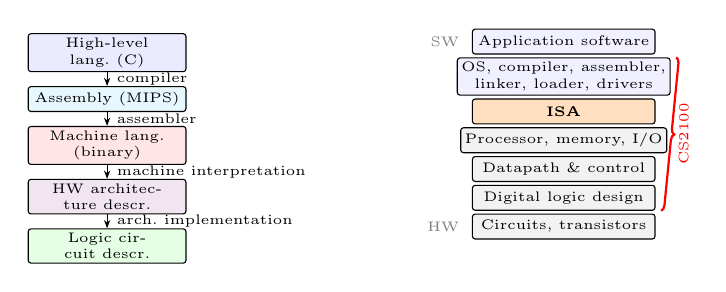
\begin{tikzpicture}[node distance=5pt,every node/.style={font=\fontsize{5.2}{5.8}\selectfont}]
 \node[box=blue!8,text width=54pt,align=center] (h) {High-level lang.\ (C)};
 \node[box=cyan!10,text width=54pt,align=center,below=of h] (a) {Assembly (MIPS)};
 \node[box=red!10,text width=54pt,align=center,below=of a] (m) {Machine lang.\ (binary)};
 \node[box=violet!10,text width=54pt,align=center,below=of m] (hw) {HW architecture descr.};
 \node[box=green!10,text width=54pt,align=center,below=of hw] (lc) {Logic circuit descr.};
 \draw[arr](h)--node[right,lbl]{compiler}(a);
 \draw[arr](a)--node[right,lbl]{assembler}(m);
 \draw[arr](m)--node[right,lbl]{machine interpretation}(hw);
 \draw[arr](hw)--node[right,lbl]{arch.\ implementation}(lc);
 \begin{scope}[xshift=165pt,yshift=4pt]
  \node[box=blue!6,minimum width=66pt] (s1) at (0,0) {Application software};
  \node[box=blue!6,minimum width=66pt,below=1pt of s1,align=center] (s2) {OS, compiler, assembler,\\linker, loader, drivers};
  \node[box=orange!25,minimum width=66pt,below=1pt of s2] (s3) {\bfseries ISA};
  \node[box=gray!10,minimum width=66pt,below=1pt of s3] (s4) {Processor, memory, I/O};
  \node[box=gray!10,minimum width=66pt,below=1pt of s4] (s5) {Datapath \& control};
  \node[box=gray!10,minimum width=66pt,below=1pt of s5] (s6) {Digital logic design};
  \node[box=gray!10,minimum width=66pt,below=1pt of s6] (s7) {Circuits, transistors};
  \draw[decorate,decoration={brace,amplitude=2pt},thick,red] ([xshift=2pt]s2.north east)--([xshift=2pt]s6.south east) node[midway,right,lbl,text=red,rotate=90,anchor=north]{CS2100};
  \node[lbl,left=1pt of s1,anchor=east,gray]{SW}; \node[lbl,left=1pt of s7,anchor=east,gray]{HW};
 \end{scope}
\end{tikzpicture}
\end{center}
Topics: C $\to$ data representation $\to$ assembly (MIPS) $\to$ datapath \& control $\to$ pipelining, cache $\to$ combinational \& sequential circuits. Tools: C debugger, QTSpim (MIPS simulator), Logisim. Textbooks: DLD (Aaron Tan), COD 4e (Patterson \& Hennessy). Final exam is open book (printed/written), calculators allowed.

\sect{L2a \; C basics: program, memory, types}
C: 1972, Dennis Ritchie, Bell Labs, for UNIX.\\
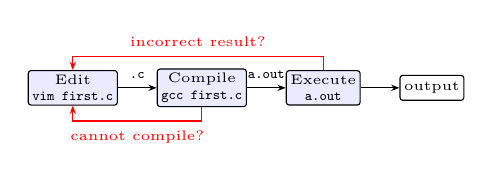
\begin{tikzpicture}[node distance=14pt]
 \node[box=blue!8,align=center] (e) {Edit\\\tc{vim first.c}};
 \node[box=blue!8,right=of e,align=center] (c) {Compile\\\tc{gcc first.c}};
 \node[box=blue!8,right=of c,align=center] (x) {Execute\\\tc{a.out}};
 \node[box=white,right=of x,align=center] (o) {output};
 \draw[arr](e)--node[above,lbl]{\tc{.c}}(c); \draw[arr](c)--node[above,lbl]{\tc{a.out}}(x); \draw[arr](x)--(o);
 \draw[arr,red](c.south)--++(0,-5pt)-|node[pos=0.25,below,lbl]{cannot compile?}(e.south);
 \draw[arr,red](x.north)--++(0,5pt)-|node[pos=0.25,above,lbl]{incorrect result?}(e.north);
\end{tikzpicture}\\
Flags: \tc{-o name} (exe name, default \tc{a.out}), \tc{-Wall} (all warnings, e.g.\ ``used uninitialized''), \tc{-lm} (link math lib), \tc{-DDEBUG}/\tc{-UDEBUG} (define/undefine macro).
\begin{lstlisting}
// Converts distance in miles to kilometres.
#include <stdio.h>        /* printf, scanf definitions */
#define KMS_PER_MILE 1.609 /* conversion constant */
int main(int argc, char *argv[]) {
  float miles, kms;                     // declarations
  printf("Enter distance in miles: ");  // input
  scanf("%f", &miles);
  kms = KMS_PER_MILE * miles;           // compute
  printf("That equals %9.2f km.\n", kms); // output
  return 0;
}
\end{lstlisting}
General form: preprocessor directives; global declarations; functions \{declarations; executable statements (input, compute, output)\}. \tc{;} ends a statement, \tc{\{\}} is a block (Python uses indentation). Comments: \tc{/* */} (only this is ANSI C) and \tc{//}. Parts of a program: preprocessor directives, reserved words, special symbols, variables, functions, comments.

\sub{von Neumann architecture} (a.k.a.\ Princeton / stored-program):\\
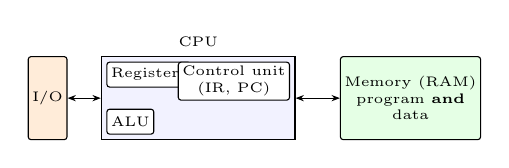
\begin{tikzpicture}
 \node[draw,fill=blue!5,minimum width=70pt,minimum height=30pt,label={[lbl]above:CPU}] (cpu) {};
 \node[box=white,anchor=north west] at ($(cpu.north west)+(2pt,-2pt)$) {Registers};
 \node[box=white,anchor=south west] at ($(cpu.south west)+(2pt,2pt)$) {ALU};
 \node[box=white,anchor=north east,align=center] at ($(cpu.north east)+(-2pt,-2pt)$) {Control unit\\(IR, PC)};
 \node[box=green!10,right=16pt of cpu,minimum height=30pt,align=center] (mem) {Memory (RAM)\\program \textbf{and}\\data};
 \node[box=orange!15,left=12pt of cpu,minimum height=30pt] (io) {I/O};
 \draw[{Stealth[length=3pt]}-{Stealth[length=3pt]}](cpu)--(mem); \draw[{Stealth[length=3pt]}-{Stealth[length=3pt]}](io)--(cpu);
\end{tikzpicture}
\warn{Uninitialised variables hold garbage, \textbf{not} 0. Before \tc{scanf}: \tc{miles=?, kms=?}; after input \tc{miles=10.5}; after compute \tc{kms=16.89}.}

\sub{Variables} have a name (identifier), a type, a value and an \emph{address}. \tc{int count = 3;} declares and initialises. Names: letters, digits, \tc{\_}; must not start with a digit; no reserved words; case-sensitive; avoid standard identifiers (\tc{printf}). Valid: \tc{maxEntries, \_X123, this\_IS\_a\_long\_name}. Invalid: \tc{1Letter, double, return, joe's, ice cream, T*S}. Redundant init: \tc{int c=0; c=123;}.

\sub{Data types} (sunfire, via \tc{sizeof}):\par
\begin{tabular}{@{}llp{150pt}l@{}}\toprule
type & bytes & notes & fmt\\\midrule
\tc{int} & 4 & $-2^{31}$ ($-2{,}147{,}483{,}648$) to $2^{31}-1$ & \tc{\%d}\\
\tc{float} & 4 & real; \tc{1.5e-2}=0.015, \tc{1.2E+5}=120000.0 & \tc{\%f}\\
\tc{double} & 8 & real (scanf needs \tc{\%lf}) & \tc{\%lf}\\
\tc{char} & 1 & \tc{'A'}, \tc{'\bs n'}, single quotes & \tc{\%c}\\\bottomrule
\end{tabular}\\
Variants: \tc{short}, \tc{long}. Strongly typed (declare type: C, Java, Pascal; Java/Pascal stronger since C allows implicit conversions and pointer casts) vs weakly typed (JS \tc{var}).

\sub{Program structure}: preprocessing directives; global declarations (\tc{struct, enum, typedef, extern}); global data definitions; global function definitions (prototype = return type, name, params; body in braces: local declarations/definitions, blocks, statements, expressions). \tc{extern int x;} = declaration vs \tc{int x;} = definition. \tc{extern int f(int a);} declaration vs \tc{int f(int a)\{...\}} definition. \emph{Parameter} = in definition (\tc{a}); \emph{argument} = in call (\tc{f(3)}). \tc{.h} files hold declarations, \tc{.c} files definitions.

\sub{Preprocessor}: (1) header inclusion \tc{\#include <stdio.h>} (I/O), \tc{<math.h>} (compile with \tc{-lm}), \tc{<string.h>}, \tc{<ctype.h>}; (2) macro expansion \tc{\#define PI 3.142} (textual replace before compiling, ALL CAPS); (3) conditional compilation \tc{\#if defined(DEBUG) ... \#endif}.

\sub{I/O} (variadic functions): \tc{printf(format, list)}, \tc{scanf(format, \&var)}. \tc{age} = value, \tc{\&age} = address of the cell (varies per run).\\
\begin{tabular}{@{}lll@{}}\toprule
spec & type & used in\\\midrule
\tc{\%c} & char & printf/scanf\\
\tc{\%d} & int & printf/scanf\\
\tc{\%f} & float or double & printf\\
\tc{\%f} & float & scanf\\
\tc{\%lf} & double & scanf\\
\tc{\%e} & float/double & printf (scientific)\\
\tc{\%p} & pointer (hex) & printf\\
\tc{\%s} & string & printf/scanf\\\bottomrule
\end{tabular}\par
\tc{\%5d}: width 5, right-justified. \tc{\%8.3f}: width 8, 3 d.p. scanf: no width/precision. Escapes: \tc{\bs n} newline, \tc{\bs t} tab, \tc{\bs "} quote, \tc{\%\%} percent.

\sect{L2b \; Compute: assignment, operators, types}
Function body = declaration statements (what memory cells) + executable statements. \tc{main} is where execution starts.\\
\sub{Assignment} \tc{=} means ``assign right to left'', \emph{not} equality. Left side is the \key{lvalue} (must be assignable): \tc{32 = a;} and \tc{a + b = c;} give ``lvalue required'' errors. Cascade is right-assoc: \tc{a = b = c = 3+6;} $\equiv$ \tc{a=(b=(c=9))}. \key{Side effect}: an assignment returns the value assigned: \tc{z = a = 12;}, \tc{a = 5 + (b = 10);} gives b=10, a=15 (legal but avoid).\\
\sub{Arithmetic} binary \tc{+ - * / \%} are left-assoc: \tc{46/15/2} $=3/2=$ \textbf{1}; \tc{19\%7\%3} $=5\%3=$ \textbf{2}. Unary \tc{+ -} right-assoc (\tc{x = -23; p = +4*10} gives 40). Order: parentheses, then precedence, then associativity; \tc{* / \%} above \tc{+ -}. Truncation on store: \tc{int n = 9*0.5;} gives \textbf{4}.

\sub{Operator precedence} (high to low):\\
\begin{tabular}{@{}p{50pt}p{95pt}l@{}}\toprule
type & operators & assoc\\\midrule
primary & \tc{() [] . -> x++ x--} & L$\to$R\\
unary & \tc{* \& + - ! \~{} ++x --x (cast) sizeof} & R$\to$L\\
multiplicative & \tc{* / \%} & L$\to$R\\
additive & \tc{+ -} & L$\to$R\\
relational & \tc{< > <= >=} & L$\to$R\\
equality & \tc{== !=} & L$\to$R\\
logical and & \tc{\&\&} & L$\to$R\\
logical or & \tc{||} & L$\to$R\\
ternary & \tc{?:} & R$\to$L\\
assignment & \tc{= += -= *= /= \%=} & R$\to$L\\\bottomrule
\end{tabular}

\sub{Mixed types \& casts}: \tc{int m=10/4}$\to$2; \tc{float p=10/4}$\to$2.0 (int division first!); \tc{float q=10/4.0}$\to$2.5; \tc{int n=10/4.0}$\to$2; \tc{int r=-10/4.0}$\to$\textbf{-2} (truncates toward 0). Cast \tc{(type) expr}: with \tc{int aa=6; float ff=15.8;} \tc{(float)aa/4}=1.5; \tc{(int)ff/aa}=15/6=2; \tc{(float)(aa/4)}=1.0.\\
\warn{C \tc{\%} is \emph{remainder} (sign follows dividend): \tc{-10\%4 = -2}. Python \tc{\%} is modulo: \tc{-10\%4 = 2}, and Python \tc{-10//4 = -3} (floor). C \tc{/} on ints truncates toward 0.}

\sect{L2c \; Selection \& repetition}
\sub{if / else; switch} (switch expression must be discrete type; falls through until \tc{break}; \tc{default} if no case matches; stack \tc{case 'A': case 'B':} to share code; GCC extension \tc{case 65 ... 67:}).\\
\sub{Conditions}: \tc{< <= > >= == !=}. No chained \tc{1<=x<=5} like Python. \key{No Boolean type in ANSI C}: 0 = false, any non-zero = true, 1 printed for true: \tc{int a=(2>3), b=(3>2);} gives a=0, b=1.\\
Logical: \tc{\&\&} and, \tc{||} or, \tc{!} not. Ternary: \tc{y = (x>0) ? x : -x;}\\
\sub{Example} \tc{a=4,b=-2,c=0}: \tc{x = (a>b || b>c \&\& a==b)} = \textbf{1} (\tc{\&\&} binds tighter: \tc{T || (F\&\&F)}); \tc{y = ((a>b || b>c) \&\& a==b)} = \textbf{0}; \tc{z = ((a>b) \&\& !(b>c))} = \textbf{1}. Add parentheses!\\
\sub{Short-circuit}: \tc{e1 || e2} skips e2 if e1 true; \tc{e1 \&\& e2} skips e2 if e1 false. So \tc{if ((a!=0) \&\& (b/a > 3))} is safe when a=0.\\
\sub{Loops}: \tc{while (c) \{\}}; \tc{do \{\} while (c);} (body runs $\ge 1$ time, note the \tc{;}); \tc{for (init; cond; update) \{\}}; \tc{for (int i=0;i<N;i++)} runs N times; \tc{for(;;)} infinite.\\
\tc{break} exits / \tc{continue} skips to next iteration of the \key{innermost} enclosing loop only. E.g.\ \tc{for i=1..5 \{print i; if(i==3) break; print "Ya"\}} prints \tc{1 Ya 2 Ya 3}; with \tc{continue}: \tc{1 Ya 2 Ya 3 4 Ya 5 Ya}. Nested (i=1..3, j=1..5, break at j==3): each i prints \tc{i,1 Ya i,2 Ya i,3} then next i.

\sect{L4a/b \; Pointers}
C is ``low'' among HLLs: pointers (direct memory manipulation) and bitwise operators.
\begin{center}
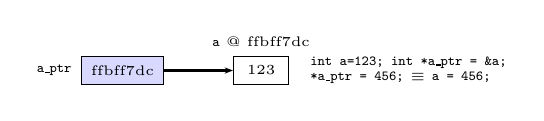
\begin{tikzpicture}[every node/.style={font=\fontsize{5.5}{6}\selectfont}]
 \node[draw,fill=blue!15,minimum width=26pt,minimum height=9pt,label={[lbl]left:\tc{a\_ptr}}] (p) {ffbff7dc};
 \node[draw,minimum width=20pt,minimum height=9pt,right=25pt of p,label={[lbl]above:\tc{a} @ ffbff7dc}] (a) {123};
 \draw[arr,thick](p)--(a);
 \node[right=4pt of a,align=left,lbl]{\tc{int a=123; int *a\_ptr = \&a;}\\\tc{*a\_ptr = 456;} $\equiv$ \tc{a = 456;}};
\end{tikzpicture}
\end{center}
\begin{itemize}
\item \tc{\&} = address-of; print with \tc{\%p} (hex, changes run to run).
\item Declare \tc{type *name;} (\tc{type} = type of pointee; suffix \tc{\_ptr}/\tc{\_p}). Only addresses can be assigned: \tc{a\_ptr = \&a;}
\item \tc{*} = indirection/dereference: \tc{*a\_ptr} is a synonym for \tc{a}.
\item \tc{double a, *b;} reads as ``\tc{*b} is a double'', so \tc{b} is a pointer to double. \tc{double *b = \&a;} OK; \tc{double b = \&a;} illegal.
\item With \tc{b=\&a; *b=12.34;}: \tc{printf("\%f",a)} and \tc{("\%f",*b)} print 12.340000; \tc{("\%f",b)} compiles with warning; \tc{("\%f",*a)} is an error; print pointer with \tc{\%p}.
\end{itemize}
\sub{Example \#1}: \tc{int i=10,j=20,*p; p=\&i; *p=*p+2;} (i=12) \tc{p=\&j; *p=i;} (j=12).\\
\sub{Trace}: \tc{a=8,b=15,c=23; p1=\&b; p2=\&c; p3=p2;} print \tc{1: 15 23 23}; \tc{*p1 *= a;} (b=120); \tc{while(*p2>0)\{*p2-=a; (*p1)++;\}} (c: 23,15,7,-1; b: 123). Prints \tc{2: 123 -1 -1} and \tc{3: 8 123 -1}.\\
\sub{Pointer arithmetic}: \tc{p++} advances by \tc{sizeof(*p)}: int +4, float +4, char +1, double +8; \tc{ap += 3} adds 12 for int.\\
\warn{\tc{int *n; *n = 123;} n points nowhere (garbage address) $\Rightarrow$ Segmentation fault (core dumped). Delete the big \tc{core} file.}
\sub{Why pointers}: let a function change caller's variables / ``return'' several values; pass an array (address of first element).

\sect{L4c/d \; Functions, pass-by-value, scope}
\sub{Library}: \tc{\#include <math.h>} + \tc{gcc -lm}. \tc{abs(int)$\to$int}; the rest take/return \tc{double}: \tc{ceil, floor, fabs, exp, log, log10, sqrt, pow(x,y), sin, cos, tan} (trig in radians). Prototype e.g.\ \tc{double pow(double x, double y)}.\\
\sub{User-defined}: put \key{prototypes} (return type, name, param types; names optional) before \tc{main}, definitions after. Without prototype the compiler assumes implicit \tc{int} return $\Rightarrow$ warning ``implicit declaration'' then error ``conflicting types''. \tc{void} function returns nothing.\\
\sub{Washer example} (rim area $=\pi(d_2/2)^2-\pi(d_1/2)^2$, volume = rim area $\times$ thickness):
\begin{lstlisting}
double circle_area(double);                 // prototype
... rim_area = circle_area(d2) - circle_area(d1);
double circle_area(double diameter) { return PI * pow(diameter/2, 2); }
\end{lstlisting}
\sub{Pass-by-value}: actual params (arguments) are \emph{copied} into formal params. Params and locals are local to the function (\key{scope rule}); an \key{activation record} is pushed on the call stack at call and popped at return, so they are \key{automatic} variables; \key{static} variables persist after the function returns. A function cannot use another function's locals (\tc{return a + x;} in \tc{f} where \tc{a} is main's: error).
\begin{center}
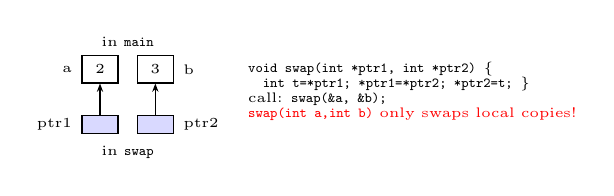
\begin{tikzpicture}[every node/.style={font=\fontsize{5.3}{6}\selectfont}]
 \node[lbl] at (0,10pt){in \tc{main}}; \node[draw,minimum width=13pt] (a) at (-10pt,0){2}; \node[draw,minimum width=13pt] (b) at (10pt,0){3};
 \node[lbl,left=0pt of a]{a}; \node[lbl,right=0pt of b]{b};
 \node[lbl] at (0,-30pt){in \tc{swap}}; \node[draw,fill=blue!15,minimum width=13pt] (p1) at (-10pt,-20pt){}; \node[draw,fill=blue!15,minimum width=13pt] (p2) at (10pt,-20pt){};
 \node[lbl,left=0pt of p1]{ptr1}; \node[lbl,right=0pt of p2]{ptr2};
 \draw[arr](p1.north)--(a.south); \draw[arr](p2.north)--(b.south);
 \node[align=left,lbl,anchor=west] at (40pt,-8pt){\tc{void swap(int *ptr1, int *ptr2) \{}\\\tc{\ \ int t=*ptr1; *ptr1=*ptr2; *ptr2=t; \}}\\ call: \tc{swap(\&a, \&b);}\\\textcolor{red}{\tc{swap(int a,int b)} only swaps local copies!}};
\end{tikzpicture}
\end{center}
\sub{Examples}: \tc{f(int x,y,z)\{x=3+y; y=10*x; z=x+y+z;\}} with a=9,b=-2,c=5: prints x=1,y=10,z=16 but a,b,c unchanged. Pointer version \tc{f(\&a,\&b,\&c)} using \tc{*x,*y,*z}: a=1,b=10,c=16. Printing \tc{x} with \tc{\%d} warns (it is an address); use \tc{\%p}.\\
\sub{Scoping}: one global scope; local scopes nest; every \tc{\{\}} makes a new scope; \key{lexical} scoping (decided at compile time from program text). Inner declaration shadows outer.
\begin{lstlisting}
int x = -1;                    // global
void foo() { printf("5. x = %d\n", x); }  // sees global: -1
int main(void) { int x; x = 10;        // 1. x = 10
  if (x > 0) { int x; x = 20; }        // 2. x = 20 (inner x)
  /* 3. x = 10 */ x = 30; /* 4. x = 30 */ foo(); /* 6. x = 30 */ }
\end{lstlisting}
\tc{static} is a storage-class specifier: on a global it limits it to \key{file scope}; on a local it changes \key{duration} (keeps value across calls). (\tc{const} is another declaration keyword.)

\sect{L5a \; Arrays}
Homogeneous collection, \key{contiguous} memory, index from 0. \tc{int c[30];} (type, name, size).
\begin{center}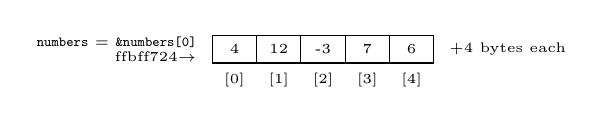
\begin{tikzpicture}[every node/.style={font=\fontsize{5}{5.5}\selectfont}]
 \foreach \i/\v in {0/4,1/12,2/-3,3/7,4/6}{\node[draw,minimum width=16pt,minimum height=8pt] (n\i) at (\i*16pt,0){\v}; \node[lbl,below=0pt of n\i]{[\i]};}
 \node[lbl,left=2pt of n0,align=right]{\tc{numbers} = \tc{\&numbers[0]}\\ffbff724$\to$};
 \node[lbl,right=2pt of n4]{+4 bytes each};
\end{tikzpicture}\end{center}
\begin{itemize}
\item Init: \tc{int a[3]=\{54,9,10\};} \tc{int b[]=\{1,2,3\};} (size 3); \tc{int c[5]=\{17,3,10\};} rest are \textbf{0}. \tc{int e[2]=\{1,2,3\};} warning (excess); \tc{f[5]=\{...\};} after declaration is a compile error.
\item Array name in an expression = address of first element (\tc{a == \&a[0]}); \tc{\&a[1]} is 4 bytes later. It is a \key{constant pointer}: \tc{dest = source;} is \textbf{illegal}; copy with a loop (or \tc{memcpy}, out of scope).
\item Parameter \tc{int arr[]} $\equiv$ \tc{int *arr}; any size inside \tc{[ ]} is ignored, so pass size separately: \tc{int sumArray(int [], int);}
\item Function receives the address $\Rightarrow$ it \key{can modify} the caller's array (no \tc{\&} needed). Use \tc{const float arr[]} to promise not to modify.
\end{itemize}

\sect{L5b \; Strings}
String = char array terminated by \tc{'\bs0'} (ASCII 0). Without it, it is just a char array.\\
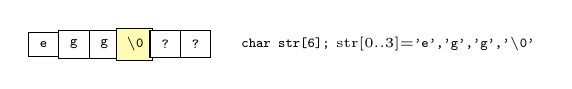
\begin{tikzpicture}[every node/.style={font=\fontsize{5.5}{6}\selectfont}]
 \foreach \i/\v/\f in {0/e/white,1/g/white,2/g/white,3/\bs0/yellow!30,4/?/white,5/?/white}{\node[draw,minimum width=11pt,minimum height=8pt,fill=\f] at (\i*11pt,0){\tc{\v}};}
 \node[lbl,anchor=west] at (68pt,0){\tc{char str[6];} str[0..3]=\tc{'e','g','g','\bs0'}};
\end{tikzpicture}\\
Init: \tc{char s[] = "apple";} (\tc{\bs0} auto-added, size 6) $\equiv$ \tc{\{'a','p','p','l','e','\bs0'\}}.\\
\sub{I/O}: \tc{fgets(str, size, stdin)} reads up to size$-1$ chars or until newline, \key{and keeps the \tc{\bs n}}: strip with \tc{len=strlen(str); if(str[len-1]=='\bs n') str[len-1]='\bs0';}. \tc{scanf("\%s",str)} stops at whitespace (input ``My book'' gives ``My''; fgets gives ``My book''). \tc{puts(str)} prints + newline; \tc{printf("\%s")}. Avoid \tc{gets} (unsafe).\\
\sub{\tc{<string.h>}}: \tc{strlen(s)} (chars before \tc{\bs0}); \tc{strcmp(s1,s2)} compares ASCII: $<0$ if s1 lexicographically smaller, $>0$ if greater, 0 if equal; \tc{strncmp(s1,s2,n)}; \tc{strcpy(s1,s2)} copies s2 into s1, returns s1 (overflows if s2 too long!); \tc{strncpy(s1,s2,n)}. \tc{name = "Matthew";} does \textbf{not} work.\\
\tc{<ctype.h>}: \tc{toupper(c)} etc. Remove-vowels: loop, \tc{switch(toupper(str[i])) \{case 'A': ... case 'U': break; default: newstr[count++]=str[i];\}} then \tc{newstr[count]='\bs0';}\\
\warn{Missing \tc{\bs0}: \tc{printf("\%s")}/\tc{strlen} run past the array until a stray 0, e.g.\ ``Length = 8, apple\textbf{??<}'' or illegal memory access.}

\sect{L5c/d \; Structures}
Heterogeneous members (fields). A \key{type} is not a variable (no memory allocated).
\begin{lstlisting}
typedef struct { int day, month, year; } date_t;
typedef struct { int cardNum; date_t expiryDate; } card_t;  // nested
typedef struct { int stuNum; float score; char grade; } result_t; // <- ; !
card_t card1 = {888888, {31, 12, 2020}};
result_t r1 = {123321, 93.5, 'A'}, r2;
r2.stuNum = 456654; card1.expiryDate.year = 2021;          // dot operator
scanf("%d %f %c", &r1.stuNum, &r1.score, &r1.grade);
r2 = r1;   // struct assignment OK (member-wise copy), unlike arrays
struct ACC { int acctNum; float balance; };  // struct tag version
struct ACC acct1, acct_arr[10];
\end{lstlisting}
Type defined by \tc{struct} itself; \tc{typedef} only names it (no new type, no variable); tag optional (anonymous \tc{struct \{int i; float b;\} x;} legal); repeated equivalent typedefs allowed (warning only). Define types after preprocessor directives, before prototypes.\\
\sub{Functions}: structs are \key{passed/returned by value} (whole struct copied): \tc{result\_t max\_and\_average(int,int,int)} returns a struct into the caller. A function receiving \tc{player\_t player} changes only its copy (``Brusco, 23'' stays). To modify, pass the address:
\begin{lstlisting}
void change_name_and_age(player_t *p) {
  strcpy(p->name, "Alexandra");  // same as (*p).name
  p->age = 25; }                 // call: change_name_and_age(&player1);
\end{lstlisting}
\warn{\tc{*p.name} means \tc{*(p.name)} since \tc{.} binds tighter than \tc{*}. Write \tc{(*p).name} or \tc{p->name}.}
Arrays of structs (e.g.\ \tc{store\_t storeList[]} with name, (x,y), radius) are passed as pointers, so functions \emph{can} modify elements.
\bigsec{secB}{L3 Number Representation \;\textbar\; L9 More on Numbers}

\sect{L3a \; Bits, bases, conversions}
Same bits, different meaning: \tc{01000110} = 70 as int, \tc{'F'} as char. \tc{0xC0D00000} = $-1060110336$ as int, $-6.5$ as float.\\
Byte = 8 bits, nibble = 4, word = multiple of bytes (arch-dependent). $N$ bits $\to 2^N$ values; $M$ values need $\lceil\log_2 M\rceil$ bits (32 values: 5 bits; 1000 values: 10 bits).\\
\sub{Weighted-positional}: $(a_n\dots a_0.f_1\dots f_m)_R=\sum a_iR^i+\sum f_jR^{-j}$. Octal digits 0 to 7, hex 0 to F.\\
Notation: C \tc{032} = octal, \tc{0x32} = hex; QTSpim \tc{0x100}; Verilog \tc{8'b11110000} = \tc{8'hF0} = \tc{8'd240}.\\
\sub{Base-R $\to$ decimal}: multiply by weights. $1101.101_2 = 8+4+1+0.5+0.125 = 13.625$; $572.6_8=378.75$; $2A.8_{16}=42.5$; $341.24_5=96.56$.\\
\sub{Decimal $\to$ base R}: whole part by \key{repeated division} by R (first remainder = LSB); fraction by \key{repeated multiplication} by R (first carry = MSB), until fraction is 0 or enough digits.\\
\begin{tabular}{@{}l|l@{}}
$43\div2$: rem 1 (LSB),1,0,1,0,1 (MSB) & $0.3125\times2=0.625\to0$ (MSB)\\
$43_{10}=101011_2$ & $0.625\to1,\ 0.25\to0,\ 0.5\to1$ (LSB)\\
 & $0.3125_{10}=.0101_2$
\end{tabular}\\
Between arbitrary bases go via decimal. \key{Shortcuts} for 2/8/16: group bits from the binary point outwards, 3 for octal, 4 for hex: $(10\,111\,011\,001.101\,110)_2=(2731.56)_8$; $(101\,1101\,1001.1011\,1000)_2=(5D9.B8)_{16}$.

\sect{L3b \; ASCII \& negative numbers}
\sub{ASCII}: 7 bits (+1 parity bit, odd or even). \tc{'0'}=48 (\tc{0x30}), \tc{'A'}=65 (\tc{0x41}), \tc{'a'}=97 (\tc{0x61}), \tc{' '}=32, \tc{'\bs0'}=0, \tc{'\bs n'}=10. Row = 3 MSBs, column = 4 LSBs: \tc{000/001} control chars, \tc{010} space and punctuation, \tc{011} digits, \tc{100/101} uppercase, \tc{110/111} lowercase. Integers 0 to 127 and chars are interchangeable in C: \tc{printf("\%c",65)}$\to$A, \tc{printf("\%d",'F')}$\to$70.\\
\sub{Past-year Q}: \tc{int n=2147483640;} add 1 ten times. After 7 adds $n=2^{31}-1$; 8th wraps to $-2147483648$; final \textbf{$-2147483646$} (32-bit 2s complement overflow).

\begin{tabular}{@{}p{34pt}p{68pt}p{84pt}p{38pt}@{}}\toprule
$n$-bit & negate & range & zeros\\\midrule
Sign-mag & flip sign bit & $-(2^{n-1}-1)$ to $2^{n-1}-1$ & $+0,-0$\\
1s comp. & invert all bits; $-x=2^n-x-1$ & $-(2^{n-1}-1)$ to $2^{n-1}-1$ & \tc{0..0}, \tc{1..1}\\
2s comp. & invert all, add 1; $-x=2^n-x$ & $-2^{n-1}$ to $2^{n-1}-1$ & one zero\\
Excess-$K$ & value $=$ code $-K$ & code 0 is $-K$ & one\\\bottomrule
\end{tabular}\\
MSB is the sign (0 +, 1 $-$) in all three signed schemes. 8-bit: s-m and 1s: $\pm127$; 2s: $-128$ to $127$.\\
E.g.\ 8-bit: $-12$: 1s \tc{11110011}, 2s \tc{11110100}. $-14$: 1s \tc{11110001}, 2s \tc{11110010}. $-80$: $80=\tc{01010000}$, 1s \tc{10101111}, 2s \tc{10110000}. s-m: \tc{00110100}=+52, \tc{10010011}=$-19$.\\
\idea{2s complement is a clock face: \tc{1111} is one step ``before'' \tc{0000}, so it is $-1$. The MSB has weight $-2^{n-1}$: $\tc{1011}=-8+2+1=-5$. Adding just goes clockwise; overflow is crossing the $+7/-8$ seam.}
\begin{center}
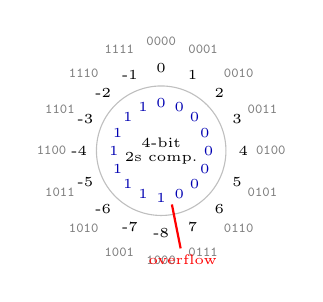
\begin{tikzpicture}[scale=0.9,every node/.style={font=\fontsize{4.8}{5}\selectfont}]
 \draw[gray!50] (0,0) circle (26pt);
 \foreach \k in {0,...,15}{
   \pgfmathtruncatemacro{\v}{\k<8 ? \k : \k-16}
   \pgfmathsetmacro{\ang}{90-\k*22.5}
   \node at (\ang:33pt) {\v};
   \node[text=blue!70!black] at (\ang:19pt) {\ifnum\k<8 0\else 1\fi};
 }
 \foreach \k/\b in {0/0000,1/0001,2/0010,3/0011,4/0100,5/0101,6/0110,7/0111,8/1000,9/1001,10/1010,11/1011,12/1100,13/1101,14/1110,15/1111}{
   \pgfmathsetmacro{\ang}{90-\k*22.5}
   \node[font=\fontsize{4}{4}\selectfont\ttfamily,gray] at (\ang:44pt) {\b};}
 \draw[red,thick] (90-7.5*22.5:22pt)--(90-7.5*22.5:40pt) node[pos=1.25,red]{overflow};
 \node[align=center] at (0,0){4-bit\\2s comp.};
\end{tikzpicture}
\hspace{4pt}
\begin{tabular}[b]{@{}c|ccc@{}}
val & s-m & 1s & 2s\\\hline
+7 & 0111&0111&0111\\
+1 & 0001&0001&0001\\
+0 & 0000&0000&0000\\
$-0$ & 1000&1111&--\\
$-1$ & 1001&1110&1111\\
$-3$ & 1011&1100&1101\\
$-5$ & 1101&1010&1011\\
$-7$ & 1111&1000&1001\\
$-8$ & -- & -- &1000
\end{tabular}
\end{center}
\sub{Fractions}: complement works too. 1s: $-0101.01 = 1010.10$, $-111000.101=000111.010$; 2s: $-0101.01 = 1010.11$ (add 1 at the last bit).\\
Complement idea: 9's complement in base 10 ($X + \bar X = 9999$).

\sect{L3c \; Add/Sub, overflow, excess}
Terms: augend + addend = sum; minuend $-$ subtrahend = difference; multiplicand $\times$ multiplier = product; dividend $\div$ divisor = quotient, remainder. $+$ and $\times$ commute; $-$ and $\div$ don't.\\
\sub{2s complement} $A+B$: add; \key{ignore carry out} of MSB; \key{overflow} iff carry-in $\ne$ carry-out of MSB, i.e.\ pos+pos=neg or neg+neg=pos. $A-B = A+(-B)$ (take 2s comp of B, add).\\
\sub{1s complement} $A+B$: add; if carry out of MSB, \key{add 1 (end-around carry)}; overflow iff result sign differs from (same) signs of A and B.\\
{\ttfamily\fontsize{5.5}{6}\selectfont
\begin{tabular}{@{}l@{\ }l|l@{\ }l@{}}
\multicolumn{2}{c|}{\rmfamily 4-bit 2s} & \multicolumn{2}{c}{\rmfamily 4-bit 1s}\\
3+4: 0011+0100=0111 & ok & 3+4 = 0111 & ok\\
-2+-6: 1110+1010=\underline{1}1000 & ok,-8 & -2+-5: 1101+1010=\underline{1}0111$\to$1000 & ok\\
6+-3: 0110+1101=\underline{1}0011 & ok & 5+-5: 0101+1010=1111 & ok (-0)\\
4+-7: 0100+1001=1101 & ok,-3 & -3+-7: 1100+1000=\underline{1}0100$\to$0101 & \textcolor{red}{OVF}\\
-3+-6: 1101+1010=\underline{1}0111 & \textcolor{red}{OVF} & & \\
5+6: 0101+0110=1011 & \textcolor{red}{OVF} & & \\
6-1: 0110+1111=\underline{1}0101 & ok,5 & & \\
-5-4: 1011+1100=\underline{1}0111 & \textcolor{red}{OVF} & &
\end{tabular}}\\
\sub{Excess-$K$} (biased): code $=$ value $+K$; spreads range evenly by translation. 3-bit excess-4: \tc{000}=$-4$ \dots\ \tc{100}=0 \dots\ \tc{111}=3. 4-bit excess-8: \tc{0000}=$-8$, \tc{1000}=0, \tc{1111}=7 (excess-7 also possible: $-7$ to 8). Codes compare like unsigned.

\sect{L3d \; Real numbers: fixed \& floating point}
\sub{Fixed point}: fixed split of integer/fraction bits (range vs precision trade-off). 8-bit, 6.2 format, 2s: \tc{011010.11} $=26.75$; \tc{111110.11}$=-000001.01=-1.25$.\\
\sub{IEEE 754} (base 2): \key{sign | exponent (biased) | mantissa}; normalised with \key{implicit leading 1} (not stored).\\
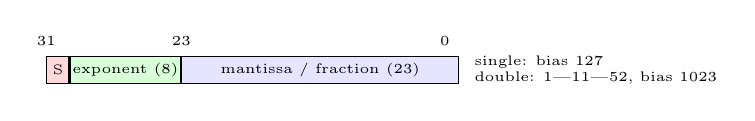
\begin{tikzpicture}[every node/.style={font=\fontsize{5.5}{6}\selectfont}]
 \node[fld,fill=red!15,minimum width=8pt] (s) at (0,0){S}; \node[fld,fill=green!15,minimum width=40pt] (e) at (s.east){exponent (8)}; \node[fld,fill=blue!10,minimum width=100pt] (m) at (e.east){mantissa / fraction (23)};
 \node[lbl,above=0pt of s.north west,anchor=south]{31}; \node[lbl,above=0pt of e.north east,anchor=south]{23}; \node[lbl,above=0pt of m.north east,anchor=south east]{0};
 \node[lbl,right=2pt of m,align=left]{single: bias 127\\double: 1|11|52, bias 1023};
\end{tikzpicture}\\
$v = (-1)^S\times 1.\text{mantissa}\times 2^{E-127}$. $110.1_2=1.101\times2^2$ (store \tc{101}); $0.00101101_2=1.01101\times2^{-3}$ (store \tc{01101}).\\
\sub{Example} $-6.5 = -110.1_2 = -1.101\times2^2$; $E=2+127=129=\tc{10000001}$: \tc{1 10000001 10100000000000000000000} $=\tc{0xC0D00000}$.\\
\sub{Recipe}: sign; convert to binary; normalise to $1.f\times2^e$; store $e+$bias; store $f$ left-aligned, pad 0s. Reverse to decode.

\sect{L9 \; More on numbers}
Everything in a computer is a finite number $\Rightarrow$ approximation $\Rightarrow$ errors that accumulate. Normalisation gives at most one bit pattern per real value (no duplicates).\\
\sub{Range}: set of distinct representable values; of interest: largest/smallest positive and negative (non-zero). \key{Overflow}: beyond largest magnitude. \key{Underflow}: non-zero value smaller in magnitude than smallest representable (no such issue for integers).\\
\sub{Precision}: min non-zero gap between two values: integers 1; fixed point $2^{-k}$ ($k$ fraction bits); floating point is \emph{relative} (depends on exponent). FP32: next number after $1.0\times2^e$ is $(1+2^{-23})\times 2^e$; about 7 to 8 decimal digits.\\
\sub{Rounding}: pick a representable result. IEEE requires computing with $\ge$3 extra bits: \key{guard}, \key{round}, \key{sticky} (OR of all bits beyond round). Extra bits arise naturally (n-bit $\times$ n-bit gives 2n bits; adding FP needs shifting one operand to align binary points). Modes: \key{round to nearest (default)}, tie: pick the one whose LSB is 0 (``to even''); toward zero; toward $+\infty$; toward $-\infty$.\\
\warn{FP arithmetic is \key{not associative}: $(A\,\text{op}\,B)\,\text{op}\,C = \text{round}(\text{round}(A\,\text{op}\,B)\,\text{op}\,C)$. Summing a list largest-first vs smallest-first generally differs. Errors propagate in long computations.}
\sub{Patriot missile (1991)}: time in tenths of a second $\times\ 0.1$ stored in 24-bit fixed point; 0.1 not exact in binary; after 100 h error $\approx0.34$ s; Scud not intercepted, 28 killed.\\
\sub{Special values} (exponent all 0s or all 1s):\\
\begin{tabular}{@{}lll@{}}\toprule
exponent & fraction & value\\\midrule
all 0 & all 0 & $\pm0$\\
all 0 & non-zero & \parbox[t]{150pt}{denormalised: $(-1)^S\times0.f\times2^{1-\text{bias}}$\\(hidden bit 0, exponent fixed at $1-$bias; tiny numbers)}\\
other & any & normalised $1.f\times2^{E-\text{bias}}$\\
all 1 & all 0 & $\pm\infty$\\
all 1 & non-zero & NaN (error)\\\bottomrule
\end{tabular}\\
\sub{AI-era formats} (LLMs have $\sim10^{12}$ parameters; low per-weight accuracy is OK, so \key{quantise}):\\
\begin{tabular}{@{}lccc l@{}}\toprule
format & bits & exp & frac & main use\\\midrule
FP64 & 64 & 11 & 52 & scientific\\
FP32 & 32 & 8 & 23 & general\\
BF16 & 16 & 8 & 7 & AI training (FP32 range)\\
FP16 & 16 & 5 & 10 & graphics, AI\\
FP8 E4M3 & 8 & 4 & 3 & weights, activations\\
FP8 E5M2 & 8 & 5 & 2 & gradients\\
FP4 E2M1 & 4 & 2 & 1 & experimental\\\bottomrule
\end{tabular}\\
Block-scaling variants: MXFP8/4, NVFP4, HiF8/4 (multi-level scale factors). \key{Integer quantisation}: scale $=(2^{b-1}-1)/\max|x|$; \tc{INT = round(x}$\times$\tc{scale)}. E.g.\ INT8, max $|x|=12.47$: scale $=127/12.47=10.18$; $-12.47\to-127$, $5.72\to58$, $8.31\to85$. INT4 less accurate than FP4, but FP4 needs HW support.
\bigsec{secC}{L6 to L8 MIPS \;\textbar\; L10 Instruction Set Architecture}

\sect{L6 \; ISA, assembly, registers}
\key{ISA} = abstraction/interface between hardware and low-level software: everything a programmer needs to make machine code work. Many implementations (cost/performance) run the same software (x86/IA-32: 80386 (1985) to Pentium 4 (2005), AMD, Transmeta).\\
C \tc{A+B} $\xrightarrow{\text{compiler}}$ \tc{add A,B} $\xrightarrow{\text{assembler}}$ \tc{1000 1100 1010 0000}. Assembly = human-readable symbolic machine code; may have \key{pseudo-instructions} (syntactic sugar, translated to $\ge1$ real instructions, e.g.\ \tc{move \$rd,\$rs} $\to$ \tc{add \$rd,\$rs,\$zero}); only real instructions count for performance.\\
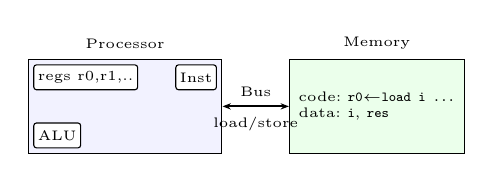
\begin{tikzpicture}[every node/.style={font=\fontsize{5.2}{5.8}\selectfont}]
 \node[draw,fill=blue!5,minimum width=70pt,minimum height=34pt,label={[lbl]above:Processor}] (p) {};
 \node[box=white,anchor=north west,align=left] at ($(p.north west)+(2pt,-2pt)$) {regs r0,r1,..};
 \node[box=white,anchor=south west] at ($(p.south west)+(2pt,2pt)$) {ALU};
 \node[box=white,anchor=north east] at ($(p.north east)+(-2pt,-2pt)$) {Inst};
 \node[draw,fill=green!8,minimum width=58pt,minimum height=34pt,right=24pt of p,align=left,label={[lbl]above:Memory}] (m) {code:\ \tc{r0$\leftarrow$load i ...}\\data:\ \tc{i}, \tc{res}};
 \draw[{Stealth[length=3pt]}-{Stealth[length=3pt]},thick](p)--node[above,lbl]{Bus}node[below,lbl]{load/store}(m);
\end{tikzpicture}\\
Walkthrough (\tc{for(i=1;i<10;i++) res+=i;}): memory is slow, so keep values in \key{registers}: \tc{r0$\leftarrow$load i; r1$\leftarrow$load res; r1$\leftarrow$r1+r0; r0$\leftarrow$r0+1; if r0<10 repeat; i$\leftarrow$store r0}. Concepts: \key{stored-program} (code+data in memory); \key{load-store} model; 3 instruction kinds: memory, calculation, control flow. Typical: load, compute, store.\\
\sub{Registers}: fast, few (16 to 32, limited by encoding), \key{no data type} (instruction decides interpretation). MIPS has 32:\\
\begin{tabular}{@{}lll|lll@{}}\toprule
name & \# & use & name & \# & use\\\midrule
\tc{\$zero} & 0 & const 0 & \tc{\$t8-\$t9} & 24-25 & more temps\\
\tc{\$at} & 1 & assembler & \tc{\$k0-\$k1} & 26-27 & OS kernel\\
\tc{\$v0-\$v1} & 2-3 & results & \tc{\$gp} & 28 & global ptr\\
\tc{\$a0-\$a3} & 4-7 & arguments & \tc{\$sp} & 29 & stack ptr\\
\tc{\$t0-\$t7} & 8-15 & temporaries & \tc{\$fp} & 30 & frame ptr\\
\tc{\$s0-\$s7} & 16-23 & program vars & \tc{\$ra} & 31 & return addr\\\bottomrule
\end{tabular}\\
(Preserved across call: \tc{\$s}, \tc{\$gp,\$sp,\$fp,\$ra}.) Other register kinds: special-purpose, FP, flag, vector, control, debug.

\sect{L6 \; Arithmetic \& logical instructions}
Syntax \tc{op dest, src1, src2}; one instruction per line; \tc{\#} comment. Arithmetic is \key{register-to-register}. Max 2 sources per instruction, so split: \tc{f=(g+h)-(i+j)} $\to$ \tc{add \$t0,\$s1,\$s2; add \$t1,\$s3,\$s4; sub \$s0,\$t0,\$t1}. Order matters for \tc{sub \$s0,\$s1,\$s2} ($\$s1-\$s2$).\\
\sub{Immediates}: \tc{addi \$s0,\$s0,4}; constant is 16-bit 2s complement $[-2^{15},2^{15}-1]$, \key{sign-extended}. No \tc{subi}: use negative \tc{addi}. \tc{\$zero} gives \tc{f=g}: \tc{add \$s0,\$s1,\$zero} (pseudo \tc{move}).\\
\sub{Logical} (register = 32 raw bits): \tc{sll}/\tc{srl} (C \tc{<<}/\tc{>>}; fill with 0; shift $n$ = $\times/\div 2^n$, e.g.\ \tc{a*8} $\to$ \tc{sll \$s0,\$s0,3}); \tc{and/andi} (\key{masking}: 1 keeps bit, 0 clears; last 12 bits: \tc{andi \$t0,\$t1,0xFFF}); \tc{or/ori} (force bits to 1); \tc{nor}; \tc{xor/xori}. C \tc{>>} is arithmetic in GCC/Clang.\\
\key{No NOT}: \tc{nor \$t0,\$t0,\$zero} or \tc{xor} with all-1s (keep ISA small). No \tc{nori} (little need) but \tc{xori} exists.\\
\warn{Logical immediates (\tc{andi, ori, xori}) are \key{zero-extended} (raw bit pattern C16); arithmetic ones (\tc{addi, slti}, offsets) are \key{sign-extended} (C16\textsubscript{2s}). \tc{ori \$t0,\$t1,0xFFFF}: upper 16 bits stay 0.}
\sub{Large constant} \tc{0xAAAAF0F0}: \tc{lui \$t0,0xAAAA} (upper 16, lower zeroed) then \tc{ori \$t0,\$t0,0xF0F0}.\\
\begin{tabular}{@{}ll|ll@{}}\toprule
instr & meaning & instr & meaning\\\midrule
\tc{add rd,rs,rt} & rd=rs+rt & \tc{addi rt,rs,C16\textsubscript{2s}} & rt=rs+C\\
\tc{sub rd,rs,rt} & rd=rs$-$rt & \tc{sll rd,rt,C5} & rd=rt$\ll$C5\\
\tc{and rd,rs,rt} & rd=rs\&rt & \tc{srl rd,rt,C5} & rd=rt$\gg$C5\\
\tc{or rd,rs,rt} & rd=rs|rt & \tc{andi rt,rs,C16} & rt=rs\&C16\\
\tc{nor rd,rs,rt} & rd=$\overline{\text{rs|rt}}$ & \tc{ori rt,rs,C16} & rt=rs|C16\\
\tc{xor rd,rs,rt} & rd=rs\^{}rt & \tc{xori rt,rs,C16} & rt=rs\^{}C16\\\bottomrule
\end{tabular}\\
C5 $\in[0,31]$ (shifting by 32 clears the register). Why learn C for MIPS: C controls memory, so C maps closely to MIPS.

\sect{L7 \; Memory, load/store}
Memory = big 1-D array of bytes (\key{byte addressing}); $k$-bit address $\Rightarrow 2^k$ locations. \key{Word} = usually $2^n$ bytes, the unit of transfer, often = register/int/instruction size. MIPS: 32 regs $\times$ 32 bits, 32-bit words and addresses, Mem[0], Mem[4], \dots, Mem[4294967292].\\
\key{Word-aligned}: address is a multiple of the word size (4): lowest 2 bits = \tc{00}.\\
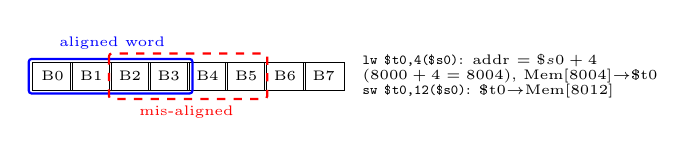
\begin{tikzpicture}[every node/.style={font=\fontsize{5}{5.5}\selectfont}]
 \foreach \i in {0,...,7}{\node[draw,minimum width=14pt,minimum height=8pt] (b\i) at (\i*14pt,0){B\i};}
 \draw[blue,thick,rounded corners=1pt]($(b0.north west)+(-1pt,1pt)$) rectangle ($(b3.south east)+(1pt,-1pt)$); \node[lbl,blue,above=1pt of b1.north east]{aligned word};
 \draw[red,thick,dashed,rounded corners=1pt]($(b2.north west)+(0,3pt)$) rectangle ($(b5.south east)+(0,-3pt)$); \node[lbl,red,below=2pt of b4.south west]{mis-aligned};
 \node[lbl,right=3pt of b7,align=left]{\tc{lw \$t0,4(\$s0)}: addr $=\$s0+4$\\ ($8000+4=8004$), Mem[8004]$\to$\$t0\\ \tc{sw \$t0,12(\$s0)}: \$t0$\to$Mem[8012]};
\end{tikzpicture}\\
\begin{itemize}
\item Only load/store touch memory; arithmetic operands must be registers.
\item \tc{A[7] = h + A[10];} (base of A in \tc{\$s3}, h in \tc{\$s2}): \tc{lw \$t0,40(\$s3); add \$t0,\$s2,\$t0; sw \$t0,28(\$s3)} (offset = index $\times$ 4).
\item \tc{lb/sb} (byte; offset need not be a multiple of 4), \tc{lh/sh}, \tc{lwl/lwr/swl/swr}. \tc{lw/sw} require aligned address; pseudo \tc{ulw/usw} for unaligned.
\item \warn{Consecutive words differ by \textbf{4}, not 1. Registers have no type: in \tc{lw \$t2,0(\$t0)}, \tc{\$t0} holds an address; in \tc{add} it holds a value.}
\end{itemize}
\sub{Swap v[k], v[k+1]} (k in \$5, base in \$4): \tc{sll \$2,\$5,2; add \$2,\$4,\$2; lw \$15,0(\$2); lw \$16,4(\$2); sw \$16,0(\$2); sw \$15,4(\$2)}.

\sect{L7 \; Branches, jumps, loops}
\tc{beq \$r1,\$r2,L} (if equal goto L), \tc{bne \$r1,\$r2,L}, \tc{j L} (always; $\equiv$ \tc{beq \$s0,\$s0,L}). Labels are anchors, not instructions. Selection = branch down; repetition = branch up.
\key{Trick}: invert the condition to skip the body.\\
\begin{minipage}[t]{0.49\linewidth}
\begin{lstlisting}[language=mips]
# if (i==j) f=g+h; else f=g-h;
      bne $s3,$s4,Else
      add $s0,$s1,$s2
      j   Exit
Else: sub $s0,$s1,$s2
Exit:
\end{lstlisting}
\end{minipage}\hfill
\begin{minipage}[t]{0.49\linewidth}
\begin{lstlisting}[language=mips]
# while (j==k) i=i+1;
Loop: bne  $s4,$s5,Exit
      addi $s3,$s3,1
      j    Loop
Exit:
\end{lstlisting}
\end{minipage}
\begin{lstlisting}[language=mips]
# for (i=0;i<10;i++) a=a+5;   i:$s0  a:$s2
      add  $s0,$zero,$zero
      addi $s1,$zero,10
Loop: beq  $s0,$s1,Exit
      addi $s2,$s2,5
      addi $s0,$s0,1
      j    Loop
Exit:
\end{lstlisting}
Decompile: \tc{beq \$s1,\$s2,Exit; add \$s0,\$zero,\$zero; Exit:} is \tc{if (i != j) f = 0;}\\
\sub{Inequalities}: \tc{slt \$t0,\$s1,\$s2} sets \tc{\$t0 = (\$s1<\$s2)?1:0}; also \tc{slti}. Pseudo \tc{blt \$s1,\$s2,L} = \tc{slt \$t0,\$s1,\$s2; bne \$t0,\$zero,L}. Others: $a>b\Leftrightarrow b<a$; $a\ge b\Leftrightarrow !(a<b)$; $a\le b\Leftrightarrow !(b<a)$.\\
\sub{Array + loop}: init counters/pointers; Label: compute address, load, work; update; compare \& branch. Count zeros in 40-word A (\tc{\$t0}=\&A, result \tc{\$t8}):
\begin{minipage}[t]{0.5\linewidth}
\begin{lstlisting}[language=mips]
# v1: index
  addi $t8,$zero,0
  addi $t1,$zero,0
  addi $t2,$zero,40
loop: bge $t1,$t2,end
  sll  $t3,$t1,2   # i*4
  add  $t4,$t0,$t3 # &A[i]
  lw   $t5,0($t4)
  bne  $t5,$zero,skip
  addi $t8,$t8,1
skip: addi $t1,$t1,1
  j loop
end:
\end{lstlisting}
\end{minipage}\hfill
\begin{minipage}[t]{0.48\linewidth}
\begin{lstlisting}[language=mips]
# v2: pointer (faster)
  addi $t8,$zero,0
  addi $t1,$t0,0    # ptr
  addi $t2,$t0,160  # &A[40]
loop: bge $t1,$t2,end
  lw   $t3,0($t1)
  bne  $t3,$zero,skip
  addi $t8,$t8,1
skip: addi $t1,$t1,4
  j loop
end:
\end{lstlisting}
\end{minipage}\\
\sub{Exercises}: counting executed instructions: count setup once, loop body $\times$ iterations, and remember the last (failing) branch. Ex\,3 (\tc{\$t1} becomes 19 so \tc{beq \$t1,\$zero,Loop} is not taken; no looping): 6 instr, \tc{\$t2}=20. Ex\,4 (\tc{bne \$t2,\$t0} with \$t2=4): 3+4$\times$3=15 instr, \$t1=0+1+2+3=6. Ex\,5 (\tc{ulw} loop from \$t0+10 down to \$t0+1): bne executed 10, taken 9, 2+4$\times$10=42 instr, bytes read $=$ offsets 1..13 $\Rightarrow$ 13 unique bytes.\\
Covered: arithmetic, large constants, load/store, branch/jump, arrays, syscalls (labs). Not covered: procedures, linker/loader, stack frames, recursion, interrupts.

\sect{L8 \; Instruction encoding (R, I, J)}
All instructions are \key{32 bits}; few, regular formats. \key{opcode} always bits 31:26; rs, rt at the same place in R and I.\\
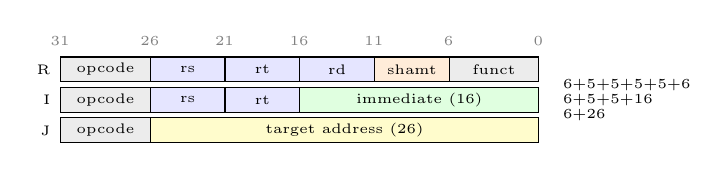
\begin{tikzpicture}[every node/.style={font=\fontsize{5.4}{6}\selectfont}]
 \def\row#1#2{\foreach \w/\t/\c [remember=\x as \lastx (initially 0)] in {#2}{\pgfmathsetmacro{\x}{\lastx+\w}\node[draw,fill=\c,minimum height=9pt,minimum width=\w*\fu,inner sep=0pt,anchor=west] at (\lastx*\fu,#1){\t};}}
 \row{0}{6/opcode/gray!15,5/rs/blue!10,5/rt/blue!10,5/rd/blue!10,5/shamt/orange!15,6/funct/gray!15}
 \row{-11pt}{6/opcode/gray!15,5/rs/blue!10,5/rt/blue!10,16/immediate (16)/green!12}
 \row{-22pt}{6/opcode/gray!15,26/target address (26)/yellow!20}
 \node[lbl,anchor=east] at (0,0){R}; \node[lbl,anchor=east] at (0,-11pt){I}; \node[lbl,anchor=east] at (0,-22pt){J};
 \foreach \b/\p in {31/0,26/6,21/11,16/16,11/21,6/26,0/32}{\node[lbl,gray,anchor=south] at (\p*\fu,5pt){\b};}
 \node[lbl,align=left,anchor=west] at (33*\fu,-11pt){6+5+5+5+5+6\\6+5+5+16\\6+26};
\end{tikzpicture}\\
\sub{R-format} (\tc{add, sub, and, or, nor, xor, slt, sll, srl}): opcode = 0; \key{funct} picks the op; rs = 1st src, rt = 2nd src, rd = dest; shamt = shift amount (0 if not a shift). Shifts: rs = 0, source in \key{rt}.\\
\sub{I-format} (\tc{addi, andi, ori, slti, lw, sw, beq, bne}): opcode alone identifies instr; rs = source; \key{rt = destination} (for arith/load). Immediate is signed except \tc{andi/ori/xori}. \tc{lw rt, C(rs)}. Branch \tc{beq rs, rt, label}: first reg is \key{rs}.\\
\sub{Examples} (fields in decimal, then hex):\\
{\ttfamily\fontsize{5.4}{6.2}\selectfont
\begin{tabular}{@{}l@{\ \ }l@{\ \ }l@{}}
add \$8,\$9,\$10 & 0|9|10|8|0|32 & 0x012A4020\\
\multicolumn{3}{@{}l}{\quad 000000 01001 01010 01000 00000 100000}\\
sll \$8,\$9,4 & 0|0|9|8|4|0 & 0x00094100\\
add \$10,\$7,\$5 & 0|7|5|10|0|32 & 0x00E55020\\
addi \$21,\$22,-50 & 8|22|21|-50 & 0x22D5FFCE\\
\multicolumn{3}{@{}l}{\quad 001000 10110 10101 1111111111001110}\\
lw \$9,12(\$8) & 35|8|9|12 & 0x8D09000C\\
beq \$9,\$0,End & 4|9|0|3 & 0x11200003
\end{tabular}}

\sub{Opcode / funct (green card)}:\\
\begin{tabular}{@{}ll|ll|ll@{}}\toprule
R (op 0) & funct & I & op & I/J & op\\\midrule
\tc{sll} & 0x00 & \tc{addi} & 0x08 & \tc{lw} & 0x23\\
\tc{srl} & 0x02 & \tc{slti} & 0x0A & \tc{sw} & 0x2B\\
\tc{jr} & 0x08 & \tc{andi} & 0x0C & \tc{lb} & 0x20\\
\tc{add} & 0x20 (32) & \tc{ori} & 0x0D & \tc{sb} & 0x28\\
\tc{sub} & 0x22 (34) & \tc{xori} & 0x0E & \tc{beq} & 0x04\\
\tc{and} & 0x24 (36) & \tc{lui} & 0x0F & \tc{bne} & 0x05\\
\tc{or} & 0x25 (37) & & & \tc{j} & 0x02\\
\tc{xor}/\tc{nor} & 0x26/0x27 & & & \tc{jal} & 0x03\\
\tc{slt} & 0x2A (42) & & & & \\\bottomrule
\end{tabular}\\
Green card: SignExtImm = \{16\{imm[15]\}, imm\}; ZeroExtImm = \{16\{0\}, imm\}; BranchAddr = \{14\{imm[15]\}, imm, 00\}; JumpAddr = \{PC+4[31:28], address, 00\}. Also \tc{jr \$ra} (jump to register), \tc{jal L} (\tc{\$ra = PC+4}, jump).

\sect{L8 \; Branch \& jump addressing}
\key{PC} holds the address of the current instruction; instructions are word-aligned.\\
\sub{Branch (PC-relative)}: loops are small, so encode an offset. Immediate counts \key{words} (instructions) from \key{PC+4}:
\[\text{not taken: } PC\leftarrow PC+4;\quad \text{taken: } PC\leftarrow (PC+4) + \text{imm}\times 4\]
Range $\pm2^{15}$ words $=\pm2^{17}$ bytes. Imm = (\#instructions between the branch and the target, counting from the one after the branch). E.g.\ \tc{beq} at 0, End at 16: imm $=(16-4)/4=3$. \tc{beq \$0,\$0,Loop} at 12 back to 0: imm $=(0-16)/4=-4$.\\
\sub{Jump (pseudo-direct)}: 26-bit field; append \tc{00} (word aligned) $\to$ 28 bits; take top 4 bits from \key{PC+4}:\\
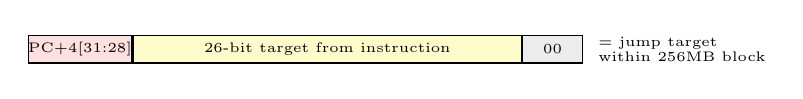
\begin{tikzpicture}[every node/.style={font=\fontsize{5.4}{6}\selectfont}]
 \node[fld,fill=red!12,minimum width=4*\fu] (a) at (0,0){PC+4[31:28]};
 \node[fld,fill=yellow!20,minimum width=26*\fu] (b) at (a.east){26-bit target from instruction};
 \node[fld,fill=gray!15,minimum width=4*\fu] (c) at (b.east){00};
 \node[lbl,right=2pt of c,align=left]{= jump target\\within 256MB block};
\end{tikzpicture}\\
Cannot jump across a 256MB boundary (\tc{0x0...}, \tc{0x1...}, \tc{0x2...}); use \tc{jr} (address in register). Example: \tc{j Loop} with Loop at 8: target field $=8/4=2$.\\
\sub{Far branch}: if L1 is out of range of \tc{beq \$s0,\$s1,L1}, use \tc{bne \$s0,\$s1,Skip; j L1; Skip:}.\\
\sub{Addressing modes (MIPS)}:
\begin{itemize}
\item \key{Register}: operand in register (\tc{add, sub, and, or, xor, nor, slt, sll, srl}).
\item \key{Immediate}: constant in instruction (\tc{addi, andi, ori, xori, slti}).
\item \key{Base/displacement}: Mem[reg + const] (\tc{lw, sw}).
\item \key{PC-relative}: (PC+4) + const$\times$4 (\tc{beq, bne}).
\item \key{Pseudo-direct}: PC[31:28] : 26 bits : 00 (\tc{j}).
\end{itemize}
Branches and load/store are both I-format but branches use PC-relative, load/store use base addressing. Shifts are R-format; other immediate instr are I-format.

\sect{L10 \; ISA design: 5 concepts}
\sub{CISC} (x86-32/IA32, VAX: polynomial-multiply instruction): complex instructions, small program size (memory was precious), complex HW, little room for optimisation. \sub{RISC} (MIPS, ARM): small simple set, easy to build/optimise HW; software combines simple ops.\\
\sub{\#1 Data storage}: where are operands and results? (von Neumann: data in memory.)\\
\begin{tabular}{@{}llll@{}}\toprule
Stack & Accumulator & Reg (load-store) & Mem-Mem\\\midrule
\tc{Push A} & \tc{Load A} & \tc{Load R1,A} & \tc{Add C,A,B}\\
\tc{Push B} & \tc{Add B} & \tc{Load R2,B} & \\
\tc{Add} & \tc{Store C} & \tc{Add R3,R1,R2} & \\
\tc{Pop C} & & \tc{Store R3,C} & \\\bottomrule
\end{tabular}\\
Stack: operands implicit on top of stack. Accumulator: one operand implicit in the accumulator (IBM 701, DEC PDP-8). GPR: only explicit operands; register-memory (Motorola 68000, Intel 80386) or register-register/load-store (MIPS, DEC Alpha). Memory-memory: all in memory (DEC VAX). \key{GPR dominates}: CPUs much faster than memory and registers plentiful; multicore needs parallelism/less memory reliance; better compilers. RISC: reg-reg; CISC: mix (IA32, for compatibility).\\
\sub{\#2 Memory \& addressing}: $k$-bit address bus $\Rightarrow 2^k$ locations; $n$-bit data bus; MAR/MDR; control lines (R/W).\\
\key{Endianness} (byte order within a word), e.g.\ \tc{0xDEADBEEF}:\\
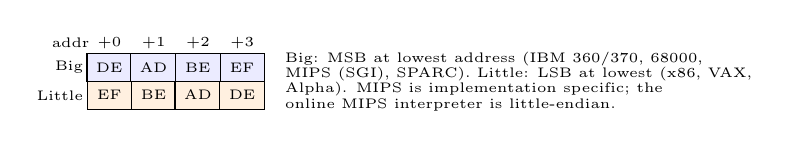
\begin{tikzpicture}[every node/.style={font=\fontsize{5.2}{5.8}\selectfont}]
 \node[lbl] at (-14pt,0){addr};
 \foreach \i in {0,...,3}{\node[lbl] at (\i*16pt,0){+\i};}
 \node[lbl,anchor=east] at (-6pt,-9pt){Big};
 \foreach \i/\v in {0/DE,1/AD,2/BE,3/EF}{\node[draw,minimum width=16pt,fill=blue!8] at (\i*16pt,-9pt){\v};}
 \node[lbl,anchor=east] at (-6pt,-19pt){Little};
 \foreach \i/\v in {0/EF,1/BE,2/AD,3/DE}{\node[draw,minimum width=16pt,fill=orange!12] at (\i*16pt,-19pt){\v};}
 \node[lbl,anchor=west,align=left] at (60pt,-14pt){Big: MSB at lowest address (IBM 360/370, 68000,\\MIPS (SGI), SPARC). Little: LSB at lowest (x86, VAX,\\Alpha). MIPS is implementation specific; the\\online MIPS interpreter is little-endian.};
\end{tikzpicture}\\
\key{Addressing modes} (MIPS has only register, immediate, displacement):\\
{\fontsize{5.6}{6.4}\selectfont\begin{tabular}{@{}lll@{}}\toprule
mode & example & meaning\\\midrule
Register & \tc{Add R4,R3} & R4$\leftarrow$R4+R3\\
Immediate & \tc{Add R4,\#3} & R4$\leftarrow$R4+3\\
Displacement & \tc{Add R4,100(R1)} & R4$\leftarrow$R4+M[100+R1]\\
Register indirect & \tc{Add R4,(R1)} & R4$\leftarrow$R4+M[R1]\\
Indexed/base & \tc{Add R3,(R1+R2)} & R3$\leftarrow$R3+M[R1+R2]\\
Direct/absolute & \tc{Add R1,(1001)} & R1$\leftarrow$R1+M[1001]\\
Memory indirect & \tc{Add R1,@(R3)} & R1$\leftarrow$R1+M[M[R3]]\\
Auto-increment & \tc{Add R1,(R2)+} & R1$\leftarrow$R1+M[R2]; R2$\leftarrow$R2+d\\
Auto-decrement & \tc{Add R1,-(R2)} & R2$\leftarrow$R2$-$d; R1$\leftarrow$R1+M[R2]\\
Scaled & \tc{Add R1,100(R2)[R3]} & R1$\leftarrow$R1+M[100+R2+R3$\times$d]\\\bottomrule
\end{tabular}}\\
\sub{\#3 Operations}: data movement (load, store, mem-mem/reg-reg move, I/O, push/pop), arithmetic (int/FP add/sub/mul/div), shift (incl.\ rotate), logical (not/and/or/set/clear), control flow (jump, branch), subroutine (call/return), interrupt (trap/return), synchronisation (test\&set, atomic r-m-w), string (search/move/compare), graphics (pixel/vertex, (de)compression).\\
\key{Frequency}: load 22\%, cond.\ branch 20\%, compare 16\%, store 12\%, add 8\%, AND 6\%, sub 5\%, move reg-reg 4\%, call 1\%, return 1\% (96\%). \key{Make the common case fast} (Amdahl): halve time of top 4 (70\%) and slow the rest by 50\%: $0.35t+0.45t=0.80t$, still a win.\\
\sub{\#4 Instruction formats}: \key{variable length} (x86: 1 to 17 bytes; VAX: 1 to 54) is compact/flexible but needs multi-step fetch/decode; \key{fixed length} (MIPS, PowerPC: 4 bytes) easy fetch/decode, simpler pipelining, but bits are scarce; \key{hybrid}. Instruction = opcode + 0 or more operands; the op designates operand type/size: char 8, half-word 16, word 32, single FP 1 word, double FP 2 words. A new 32-bit ISA should support 8/16/32-bit ints and 32/64-bit FP (64-bit ISA: 64-bit ints too).\\
\sub{\#5 Encoding}: trade-offs between code size, speed, complexity; decide \#registers, \#addressing modes, \#operands. Forces: many regs and modes vs small code vs easy (fixed) length. Choices: variable (VAX, x86), fixed (Alpha, ARM, MIPS, PowerPC, SPARC, SuperH), hybrid (IBM 360/70, MIPS16, Thumb, TI TMS320C54x).\\
\key{Expanding opcode}: opcode length varies by instruction type (MIPS \tc{funct} is an example); design the most constrained type (needs most operand bits) first.\\
\idea{Expanding opcode is like prefix-free phone numbers: reserve some short opcodes as ``escape'' prefixes, then the freed operand bits extend the opcode for instructions that need fewer operands. Count: if $k$ opcode patterns are used by type A, the remaining $2^n-k$ patterns each expand by the extra bits for type B.}
To learn any ISA: data storage, addressing modes, operations, formats, encoding (+ assembler conventions; procedures/stack and privileged instructions not covered).

\sect{C $\to$ MIPS compilation patterns (L7 advice: learn these)}
Rewrite the construct with \tc{if (...) goto}, invert the condition, then map \tc{==}/\tc{!=} to \tc{beq}/\tc{bne}, \tc{<} to \tc{slt}+\tc{bne}/\tc{beq}.\\
\begin{minipage}[t]{0.5\linewidth}
\begin{lstlisting}[language=mips]
# do { body } while (a != b);
Loop: <body>
      bne  $a,$b,Loop

# if (a < b) X;
      slt  $t0,$a,$b
      beq  $t0,$zero,Skip
      <X>
Skip:
\end{lstlisting}
\end{minipage}\hfill
\begin{minipage}[t]{0.48\linewidth}
\begin{lstlisting}[language=mips]
# while (a < b) body;
Loop: slt  $t0,$a,$b
      beq  $t0,$zero,Exit
      <body>
      j    Loop
Exit:
# if (a >= b) X;  == !(a<b)
      slt  $t0,$a,$b
      bne  $t0,$zero,Skip
\end{lstlisting}
\end{minipage}
\begin{itemize}
\item \tc{for(init;cond;upd) body} $\equiv$ \tc{init; while(cond)\{body; upd;\}}.
\item Array \tc{A[i]} (words): \tc{sll \$t,\$i,2; add \$t,\$base,\$t; lw \$x,0(\$t)}. Constant index $k$: \tc{lw \$x,4k(\$base)}. Bytes (\tc{char}): no scaling, use \tc{lb/sb}.
\item Instruction counting: total = setup + (iterations $\times$ body) + final exit check.
\end{itemize}

\sect{Quick reference: formulas}
{\fontsize{5.8}{6.6}\selectfont
\begin{tabular}{@{}p{58pt}p{110pt}@{}}\toprule
$n$-bit unsigned & $0$ to $2^n-1$\\
$n$-bit 2s comp & $-2^{n-1}$ to $2^{n-1}-1$\\
$n$-bit s-m / 1s & $-(2^{n-1}-1)$ to $2^{n-1}-1$\\
1s negate & $2^n - x - 1$ (invert)\\
2s negate & $2^n - x$ (invert, +1)\\
IEEE single & $(-1)^S 1.f\times 2^{E-127}$\\
IEEE double & bias 1023, 1+11+52\\
branch target & $(PC+4)+\text{imm}\times4$\\
jump target & PC+4[31:28] $\|$ addr26 $\|$ 00\\
imm range & addi: $[-2^{15},2^{15}-1]$; shamt $[0,31]$\\
lw/sw offset & index $\times$ 4 (words)\\\bottomrule
\end{tabular}}
\end{multicols*}
\newpage
\colorlet{cur}{secD}
\bigsec{secD}{L11 Datapath \;\textbar\; L12 Control \;\textbar\; single-cycle MIPS (supports add, sub, and, or, slt, lw, sw, beq; +addi, bne in principle)}
\vspace{2pt}
\noindent
\begin{minipage}[t]{0.575\textwidth}\vspace{0pt}
\centering
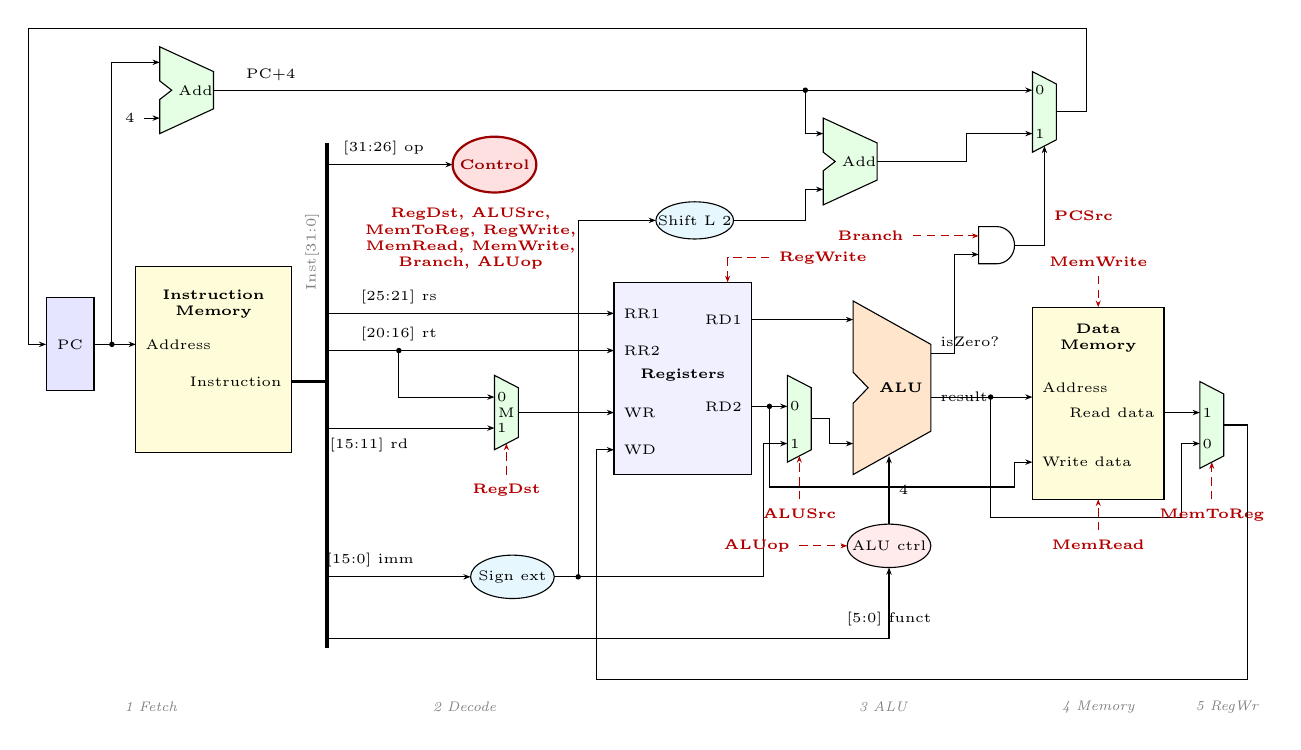
\begin{tikzpicture}[x=1.08pt,y=1.12pt,>=Stealth,
  every node/.style={font=\fontsize{5.3}{5.8}\selectfont},
  w/.style={thin,-{Stealth[length=2.6pt]}},
  ctl/.style={red!70!black,densely dashed,-{Stealth[length=2.4pt]}},
  sig/.style={text=red!70!black,font=\fontsize{5.3}{5.8}\selectfont\bfseries},
  dot/.style={circle,fill,inner sep=0.7pt}]
 % ---- PC & instruction memory
 \draw[fill=blue!10] (10,105) rectangle (26,135); \node at (18,120){PC};
 \draw[fill=yellow!15] (40,85) rectangle (92,145); \node[align=center] at (66,133){\bfseries Instruction\\\bfseries Memory};
 \node[anchor=west] at (40,120){Address}; \node[anchor=east] at (92,108){Instruction};
 \draw[w](26,120)--(40,120);
 % ---- PC+4 adder
 \draw[fill=green!10] (48,188)--(66,196)--(66,208)--(48,216)--(48,205)--(52,202)--(48,199)--cycle; \node at (60,202){Add};
 \draw[w](32,120) node[dot]{}--(32,211)--(48,211);
 \node(four) at (38,193){4}; \draw[w](four)--(48,193);
 \draw[w](66,202)--(340,202) node[pos=0.07,above]{PC+4};
 % ---- instruction bus and fields
 \draw[very thick](92,108)--(104,108); \draw[very thick](104,22)--(104,185);
 \node[rotate=90,gray] at (99,150){Inst[31:0]};
 \draw[w](104,178)--(146,178) node[pos=0.45,above]{[31:26] op};
 \draw[w](104,130)--(200,130) node[pos=0.25,above]{[25:21] rs};
 \draw[w](104,118)--(200,118) node[pos=0.25,above]{[20:16] rt};
 \draw[w](128,118) node[dot]{}--(128,103)--(160,103);
 \draw[w](104,93)--(160,93) node[pos=0.25,below]{[15:11] rd};
 \draw[w](104,45)--(152,45) node[pos=0.3,above]{[15:0] imm};
 \draw[w](104,25)--(292,25)--(292,48) node[pos=0.05,above]{[5:0] funct};
 % ---- control
 \draw[fill=red!12,thick,draw=red!60!black] (160,178) ellipse (14 and 9); \node[red!60!black] at (160,178){\bfseries Control};
 \node[sig,anchor=north,align=center] at (152,167){RegDst, ALUSrc,\\MemToReg, RegWrite,\\MemRead, MemWrite,\\Branch, ALUop};
 % ---- RegDst mux
 \draw[fill=green!10](160,86)--(168,90)--(168,106)--(160,110)--cycle; \node at (164,98){\tiny M};
 \node[font=\fontsize{4}{4}\selectfont] at (162.5,103){0}; \node[font=\fontsize{4}{4}\selectfont] at (162.5,93){1};
 \draw[w](168,98)--(200,98);
 \draw[ctl](164,78) node[below,sig]{RegDst}--(164,88);
 % ---- register file
 \draw[fill=blue!6] (200,78) rectangle (246,140); \node[align=center] at (223,110){\bfseries Registers};
 \node[anchor=west] at (200,130){RR1}; \node[anchor=west] at (200,118){RR2}; \node[anchor=west] at (200,98){WR}; \node[anchor=west] at (200,86){WD};
 \node[anchor=east] at (246,128){RD1}; \node[anchor=east] at (246,100){RD2};
 \draw[ctl](252,148) node[right,sig]{RegWrite}--(238,148)--(238,140);
 % ---- sign extend
 \draw[fill=cyan!10](166,45) ellipse (14 and 7); \node at (166,45){Sign ext};
 \draw[w](180,45)--(250,45)--(250,88)--(258,88); \node[dot] at (188,45){};
 % ---- shift left 2
 \draw[w](188,45)--(188,160)--(214,160);
 \draw[fill=cyan!10](227,160) ellipse (13 and 6); \node at (227,160){Shift L 2};
 % ---- branch adder
 \draw[fill=green!10] (270,165)--(288,173)--(288,185)--(270,193)--(270,182)--(274,179)--(270,176)--cycle; \node at (282,179){Add};
 \draw[w](264,202) node[dot]{}--(264,188)--(270,188);
 \draw[w](240,160)--(264,160)--(264,170)--(270,170);
 \draw[w](288,179)--(318,179)--(318,188)--(340,188);
 % ---- PCSrc mux
 \draw[fill=green!10](340,182)--(348,186)--(348,204)--(340,208)--cycle;
 \node[font=\fontsize{4}{4}\selectfont] at (342.5,202){0}; \node[font=\fontsize{4}{4}\selectfont] at (342.5,188){1};
 \draw[w](348,195)--(358,195)--(358,222)--(4,222)--(4,120)--(10,120);
 % ---- ALUSrc mux
 \draw[w](246,100)--(258,100); \node[dot] at (252,100){};
 \draw[fill=green!10](258,82)--(266,86)--(266,106)--(258,110)--cycle;
 \node[font=\fontsize{4}{4}\selectfont] at (260.5,100){0}; \node[font=\fontsize{4}{4}\selectfont] at (260.5,88){1};
 \draw[ctl](262,70) node[below,sig]{ALUSrc}--(262,84);
 % ---- ALU
 \draw[fill=orange!20](280,78)--(306,92)--(306,120)--(280,134)--(280,111)--(285,106)--(280,101)--cycle; \node at (296,106){\bfseries ALU};
 \draw[w](246,128)--(280,128);
 \draw[w](266,96)--(272,96)--(272,88)--(280,88);
 \node[anchor=west] at (306,121){isZero?}; \node[anchor=west] at (306,103){result};
 % ---- ALU control
 \draw[fill=red!8](292,55) ellipse (14 and 7); \node at (292,55){ALU ctrl};
 \draw[w](292,62)--(292,84) node[pos=0.5,right]{4};
 \draw[ctl](262,55) node[left,sig]{ALUop}--(278,55);
 % ---- branch AND
 \draw[fill=white](322,146)--(328,146) arc (-90:90:6)--(322,158)--cycle;
 \draw[w](306,117)--(314,117)--(314,149)--(322,149);
 \draw[ctl](300,155) node[left,sig]{Branch}--(322,155);
 \draw[w](334,152)--(344,152)--(344,184) node[pos=0.3,right,sig]{PCSrc};
 % ---- data memory
 \draw[fill=yellow!15] (340,70) rectangle (384,132); \node[align=center] at (362,122){\bfseries Data\\\bfseries Memory};
 \node[anchor=west] at (340,106){Address}; \node[anchor=west] at (340,82){Write data}; \node[anchor=east] at (384,98){Read data};
 \draw[w](306,103)--(340,103); \node[dot] at (326,103){};
 \draw[w](252,100)--(252,74)--(334,74)--(334,82)--(340,82);
 \draw[ctl](362,142) node[above,sig]{MemWrite}--(362,132);
 \draw[ctl](362,60) node[below,sig]{MemRead}--(362,70);
 % ---- MemToReg mux
 \draw[fill=green!10](396,80)--(404,84)--(404,104)--(396,108)--cycle;
 \node[font=\fontsize{4}{4}\selectfont] at (398.5,98){1}; \node[font=\fontsize{4}{4}\selectfont] at (398.5,88){0};
 \draw[w](384,98)--(396,98);
 \draw[w](326,103)--(326,64)--(390,64)--(390,88)--(396,88);
 \draw[ctl](400,70) node[below,sig]{MemToReg}--(400,82);
 \draw[w](404,94)--(412,94)--(412,12)--(194,12)--(194,86)--(200,86);
 % ---- stage labels
 \foreach \x/\t in {45/1 Fetch,150/2 Decode / Operand fetch,290/3 ALU,362/4 Memory,405/5 RegWr}{\node[gray,font=\fontsize{5}{5}\selectfont\itshape] at (\x,3){\t};}
\end{tikzpicture}
\end{minipage}\hfill
\begin{minipage}[t]{0.415\textwidth}\vspace{0pt}
\colorlet{cur}{secD}
{\color{secD}\bfseries Control signals (L12)}\\[1pt]
{\fontsize{5.6}{6.4}\selectfont
\begin{tabular}{@{}l l p{80pt} p{95pt}@{}}\toprule
signal & stage & 0 (false) & 1 (true)\\\midrule
RegDst & Decode & WR = Inst[20:16] (rt) & WR = Inst[15:11] (rd)\\
RegWrite & Dec/RegWr & no register write & write WD into register WR\\
ALUSrc & ALU & op2 = RD2 (register) & op2 = SignExt(Inst[15:0])\\
ALUcontrol & ALU & \multicolumn{2}{l}{4-bit: selects ALU operation (table below)}\\
MemRead & Memory & no memory read & read Mem[Address]\\
MemWrite & Memory & no memory write & Mem[Address] $\leftarrow$ RD2\\
MemToReg & RegWrite & WD = ALU result & WD = memory read data\\
PCSrc & Mem/RegWr & PC $\leftarrow$ PC+4 & PC $\leftarrow$ (PC+4) + SignExt(imm)$\ll$2\\\bottomrule
\end{tabular}
\warn{MemToReg mux has its inputs \textbf{swapped} (1 on top = memory). \key{PCSrc = Branch AND isZero}.}
\textbf{Main control truth table} (input: opcode Inst[31:26]):\\
\begin{tabular}{@{}l l|c c c c c c c|c c@{}}\toprule
 & opcode & RegDst & ALUSrc & MemToReg & RegWr & MemRd & MemWr & Branch & op1 & op0\\\midrule
R-type & 000000 (0) & 1 & 0 & 0 & 1 & 0 & 0 & 0 & 1 & 0\\
lw & 100011 (23) & 0 & 1 & 1 & 1 & 1 & 0 & 0 & 0 & 0\\
sw & 101011 (2B) & X & 1 & X & 0 & 0 & 1 & 0 & 0 & 0\\
beq & 000100 (4) & X & 0 & X & 0 & 0 & 0 & 1 & 0 & 1\\\bottomrule
\end{tabular}\\
One AND gate per opcode (R-format, lw, sw, beq), then OR where needed: RegDst = ALUop1 = R-format; ALUSrc = lw + sw; MemToReg = MemRead = lw; RegWrite = R-format + lw; MemWrite = sw; Branch = ALUop0 = beq.\\[2pt]
\textbf{ALU control} (2-level: opcode$\to$ALUop; ALUop + funct$\to$ALUcontrol):\\
\begin{tabular}[t]{@{}l c c c c@{}}\toprule
instr & ALUop & funct & action & ALUctrl\\\midrule
lw, sw & 00 & XXXXXX & add & 0010\\
beq & 01 & XXXXXX & subtract & 0110\\
add & 10 & 100000 & add & 0010\\
sub & 10 & 100010 & subtract & 0110\\
and & 10 & 100100 & AND & 0000\\
or & 10 & 100101 & OR & 0001\\
slt & 10 & 101010 & slt & 0111\\\bottomrule
\end{tabular}\hfill
\begin{tabular}[t]{@{}l|c c c@{}}\toprule
ALUcontrol & Ainv & Binv & Op\\\midrule
AND 0000 & 0&0&00\\ OR 0001 &0&0&01\\ add 0010 &0&0&10\\ sub 0110&0&1&10\\ slt 0111&0&1&11\\ NOR 1100&1&1&00\\\bottomrule
\end{tabular}\\[1pt]
ALUcontrol3 = 0;\quad ALUcontrol2 = ALUop0 + ALUop1$\cdot$F1;\\
ALUcontrol1 = $\overline{\text{ALUop1}}$ + $\overline{\text{F2}}$;\quad ALUcontrol0 = ALUop1$\cdot$(F3 + F0).\\
(ALUop 11 never occurs, so ALUop1 alone flags R-type (the beq row's MSB becomes X); F5, F4 are 10 for all these, so ignored.)
}
\end{minipage}

\vspace{3pt}
\begin{multicols}{3}
\sect{L11 \; Datapath basics}
Processor = \key{datapath} (components that process data: arithmetic, logic, memory ops) + \key{control} (tells datapath, memory, I/O what to do per instruction). Implements subset: \tc{add, sub, and, or, addi, andi, ori, slt}, \tc{lw, sw}, \tc{beq, bne}. \tc{andi/ori} are \textbf{not} truly supported here since the immediate is always \emph{sign}-extended. \tc{sll/srl} and \tc{j} not supported (shift = repeated add; \tc{j} $\approx$ \tc{beq \$zero,\$zero,L} ignoring 256MB blocks).\\
\sub{Instruction cycle}: Fetch $\to$ Decode $\to$ Operand fetch $\to$ Execute $\to$ Result write (each stage's output feeds the next). MIPS: merge Decode + Operand fetch (decoding is simple), split Execute into ALU + Memory $\Rightarrow$ \key{Fetch, Decode, ALU, Memory, RegWrite}.\\
{\fontsize{5.6}{6.4}\selectfont\begin{tabular}{@{}p{28pt}p{55pt}p{65pt}p{85pt}@{}}\toprule
 & \tc{add rd,rs,rt} & \tc{lw rt,ofst(rs)} & \tc{beq rs,rt,ofst}\\\midrule
Decode & opr1=[rs], opr2=[rt] & opr1=[rs], opr2=ofst & opr1=[rs], opr2=[rt]\\
ALU & opr1+opr2 & MemAddr=opr1+opr2 & Taken=(opr1==opr2); Target=(PC+4)+ofst$\times$4\\
Memory & idle & read Mem[MemAddr] & idle\\
RegWrite & $\to$ rd & mem data $\to$ rt & if Taken, PC=Target\\\bottomrule
\end{tabular}}
\sect{L11 \; Stage by stage}
\sub{1 Fetch}: read instruction at PC from \key{instruction memory}; PC $\leftarrow$ PC+4 via an adder (next instruction is 4 bytes on, except branch/jump). Output: the instruction.\\
\key{Clocking}: PC is read during the clock period; the new value is written at the next \key{rising edge} (must be ready before it). Between edges PC is stable.\\
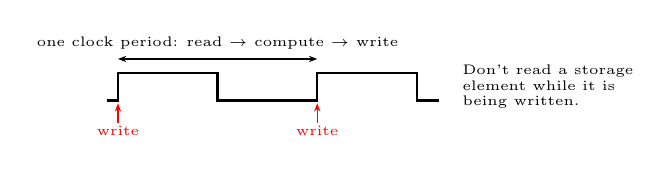
\begin{tikzpicture}[every node/.style={font=\fontsize{5}{5.5}\selectfont}]
 \draw[thick] (0,0)--(4pt,0)--(4pt,10pt)--(40pt,10pt)--(40pt,0)--(76pt,0)--(76pt,10pt)--(112pt,10pt)--(112pt,0)--(120pt,0);
 \draw[red,-{Stealth[length=3pt]}](4pt,-8pt)--(4pt,-1pt); \draw[red,-{Stealth[length=3pt]}](76pt,-8pt)--(76pt,-1pt);
 \node[red] at (4pt,-11pt){write}; \node[red] at (76pt,-11pt){write};
 \draw[{Stealth[length=3pt]}-{Stealth[length=3pt]}](4pt,15pt)--(76pt,15pt) node[midway,above]{one clock period: read $\to$ compute $\to$ write};
 \node[anchor=west,align=left] at (125pt,5pt){Don't read a storage\\element while it is\\being written.};
\end{tikzpicture}\\
Elements as functions: \tc{IM(addr)=Mem[addr]}; \tc{Add(A,B)=A+B} (combinational); instruction memory is sequential (has state; clock implied).\\
\sub{2 Decode}: split instruction \tc{Inst[Y:X]} = bits X..Y: op [31:26], rs [25:21], rt [20:16], rd [15:11], shamt [10:6], funct [5:0], imm [15:0]. \key{Register file}: 32$\times$32-bit; reads $\le$2 (RR1$\to$RD1, RR2$\to$RD2), writes $\le$1 (WR, WD) when \key{RegWrite}=1.\\
Problems for I-format (\tc{addi \$21,\$22,-50}): destination is in rt (not rd) $\Rightarrow$ \key{RegDst mux}; operand 2 is the immediate $\Rightarrow$ \key{sign-extend} 16$\to$32 bits and \key{ALUSrc mux}. \tc{lw} needs nothing extra here. \tc{beq}: outcome and target both needed, solved in ALU stage.\\
\key{Multiplexer}: $n=2^m$ inputs of equal width, $m$ control bits, output = input$_i$ when control $=i$. Larger muxes are built from 2-input ones.\\
\sub{3 ALU} (execute): arithmetic, shift, logic; address calculation for \tc{lw/sw}; compare + target for branches. ALU: two 32-bit inputs, 4-bit \key{ALUcontrol}, outputs result and 1-bit \key{isZero?} (result==0). \tc{beq}: subtract, isZero=1 means equal (\tc{bne}: taken when isZero=0). Branch target needs an extra adder: (PC+4) + (SignExt(imm) $\ll$ 2) and a \key{PCSrc mux}.\\
\sub{4 Memory}: only \tc{lw/sw} use it; address from ALU. \key{Data memory}: Address, Write data (= RD2, for \tc{sw}), Read data (for \tc{lw}); \key{MemRead}/\key{MemWrite}, at most one asserted. Others idle; ALU result passes through.\\
\sub{5 RegWrite}: route result (ALU or memory, chosen by \key{MemToReg} mux) to WD; WR number was chosen back in Decode. Stores, branches, jumps write nothing.

\sect{L12 \; Control design}
Signals derived from the \key{opcode} (format) and, for R-type, \key{funct}. All signals except ALUcontrol come from opcode alone $\Rightarrow$ most of the controller is opcode-only. Steps: list instruction subset; for each signal see how it depends on op/funct; build truth table; design with gates.\\
Subset: R-type (op 0; funct add 20, sub 22, and 24, or 25, slt 2A hex), \tc{lw} 23, \tc{sw} 2B, \tc{beq} 4.\\
\sub{1-bit ALU} (ALU built one bit at a time): 4 control bits = Ainvert, Binvert, Operation (2 bits) selecting AND / OR / sum (/ less for slt).\\
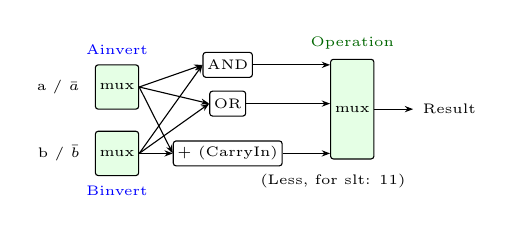
\begin{tikzpicture}[every node/.style={font=\fontsize{5}{5.5}\selectfont}]
 \node[box=green!10,minimum height=16pt] (ma) at (10pt,22pt){mux};
 \node[box=green!10,minimum height=16pt] (mb) at (10pt,-2pt){mux};
 \node[lbl,left=2pt of ma,align=right]{a / $\bar a$}; \node[lbl,left=2pt of mb,align=right]{b / $\bar b$};
 \node[lbl,above=0pt of ma,blue]{Ainvert}; \node[lbl,below=0pt of mb,blue]{Binvert};
 \node[box=white] (and) at (50pt,30pt){AND}; \node[box=white] (or) at (50pt,16pt){OR}; \node[box=white] (add) at (50pt,-2pt){+ (CarryIn)};
 \foreach \g in {and,or,add}{\draw[arr](ma.east)--(\g.west); \draw[arr](mb.east)--(\g.west);}
 \node[box=green!10,minimum height=36pt] (mo) at (95pt,14pt){mux};
 \draw[arr](and)--(mo.west|-and); \draw[arr](or)--(mo.west|-or); \draw[arr](add)--(mo.west|-add);
 \node[lbl,above=0pt of mo,green!40!black]{Operation}; \draw[arr](mo)--++(22pt,0) node[right,lbl]{Result};
 \node[lbl] at (88pt,-12pt){(Less, for slt: 11)};
\end{tikzpicture}\\
Subtract = Binvert + CarryIn 1 (2s comp); NOR = $\bar a\cdot\bar b$ (Ainvert, Binvert, AND). \key{Multilevel decoding}: instead of a 12-input function (op+funct), first opcode $\to$ 2-bit \key{ALUop} (00 lw/sw, 01 beq, 10 R-type), then ALUop+funct $\to$ ALUcontrol. Simpler design, smaller main controller, potentially faster.

\sect{L12 \; Instruction execution \& performance}
Every instruction in one clock period: (1) read storage (regs/memory), (2) compute via combinational logic, (3) write storage. Datapath shared by instruction types via MUXes + control signals generated from the encoding.\\
\sub{Single-cycle shortcoming} (memory 2ns, ALU/adders 2ns, register file 1ns):\\
\begin{tabular}{@{}lcccccc@{}}\toprule
instr & IMem & RegRd & ALU & DMem & RegWr & total\\\midrule
ALU & 2 & 1 & 2 & & 1 & 6\\
lw & 2 & 1 & 2 & 2 & 1 & \textbf{8}\\
sw & 2 & 1 & 2 & 2 & & 7\\
beq & 2 & 1 & 2 & & & 5\\\bottomrule
\end{tabular}\\
Clock must fit the slowest (\tc{lw}, 8ns) so every instruction takes 8ns.\\
\key{Fix 1: multicycle}: one step (fetch, decode/reg read, ALU, mem, reg write) per clock; shorter cycle, higher frequency; instructions take variable \#cycles (COD 5.5, not covered). \key{Fix 2: pipelining}: steps as above, but different instructions occupy different steps simultaneously (later lecture).

\sect{Tracing tips (exam style)}
\begin{itemize}
\item For a given instruction, walk the 5 stages and read off each mux select: e.g.\ \tc{sw \$21,-50(\$22)}: RegDst X, ALUSrc 1, ALUop 00 (add), MemWrite 1, RegWrite 0, MemToReg X, Branch 0.
\item Value on a wire: RD1 = [rs]; RD2 = [rt]; SignExt(imm); ALU result = address for lw/sw; branch target = PC+4+imm$\times$4.
\item X (don't care) appears when the result of that mux is never written/used (RegDst, MemToReg for sw/beq).
\item \tc{bne} needs Branch AND $\overline{\text{isZero}}$ (an extra signal). \tc{addi} would be like lw without memory: RegDst 0, ALUSrc 1, MemToReg 0, RegWrite 1, ALUop 00.
\end{itemize}

\end{multicols}
\end{document}